\documentclass{amsart}
\usepackage{amsmath}
\usepackage{amssymb}
\usepackage{amsfonts}
\usepackage{amsthm}
%% \usepackage{amsaddr}


\usepackage{thm-restate}
\usepackage{tikz,pgfplotstable}
\usetikzlibrary{patterns}
\pgfplotsset{compat=1.9} % set to 1.8 to get old behaviour
%\usepackage{hyperref}
\usepackage{xcolor}

\newcommand{\R}{\ensuremath{\mathbb{R}}}
\newcommand{\eps}{\varepsilon}
\newcommand{\M}{\mathcal{M}}

\newcommand{\der}{\text{\textup{d}}}
\newcommand{\diag}{\textup{diag}}

\providecommand{\x}{}
\renewcommand{\x}{\mathbf{x}}
\newcommand{\y}{\mathbf{y}}

\newcommand{\hil}{\mathcal{H}}
\newcommand{\hilp}{\mathcal{H}_p}
\newcommand{\hilo}{\mathcal{H}_o}
\newcommand{\obs}{\mathcal{O}}
\newcommand{\pobs}{\mathcal{P}}
\newcommand{\fwd}{\mathcal{F}}

\newcommand{\obsm}{\widehat{\obs}}
\newcommand{\Sigmam}{\widehat{\Sigma}}
\newcommand{\postcovm}{\widehat{\Gamma_{\textup{post}}}}
\newcommand{\uu}{\mathbf{u}}
\newcommand{\tar}{\Psi}
\DeclareMathOperator*{\argmin}{arg\,min}
\DeclareMathOperator*{\argmax}{arg\,max}
\DeclareMathOperator*{\conv}{conv}


% Definitions for second chapter
\newcommand{\data}{\mathbf{d}}
\newcommand{\param}{\mathbf{m}}
\newcommand{\normal}{\mathcal{N}}
\newcommand{\pr}{\mu_{\textup{pr}}} %Prior measure
%\newcommand{\post}{\mu_{\textup{post}}^{\data, \obs}} % Posterior measure
\newcommand{\post}{\mu_{\textup{post}}} % Posterior measure for slides
\newcommand{\prmean}{\param_{\textup{pr}}} % Prior mean
\newcommand{\postmean}{\param_{\textup{post}}} % Posterior mean
\newcommand{\postcov}{\Gamma_{\textup{post}}} % Posterior covariance
\newcommand{\prcov}{\Gamma_{\textup{pr}}} % Prior covariance
\newcommand{\modcov}{\Gamma_{\textup{model}}} % Model covariance
\newcommand{\tmp}{\mathcal{G}}
\newcommand{\meas}{\mathbf{o}}
\newcommand{\ev}{\mathbf{e}} % eigenvector 
\newcommand{\func}{\mathbf{a}}
\newcommand{\tr}[1]{\textup{tr}\left \{#1 \right \} }
\newcommand{\ttr}[1]{\textup{tr}\ #1}
\newcommand{\rank}{\textup{rank}\ }
\newcommand{\des}{\eta} % vector of design parameters
\newcommand{\sigsqr}{\sigma^2}

%% \newcommand{\opt}{\mathfrak{D}}
\newcommand{\opt}{\mathcal{D}}
\newcommand{\postopt}{\mu_{\textup{post}}^{\data, \opt}} % Posterior measure

%% %\usepackage{comment}% http://ctan.org/pkg/comment
%% %% %% %\excludecomment{proof}
%% %% \excludecomment{figure}
%% %% \let\endfigure\relax


%% %\overfullrule=0pt

\theoremstyle{plain}
\newtheorem{theorem}{Theorem}
\newtheorem{corollary}[theorem]{Corollary}
\newtheorem{lemma}[theorem]{Lemma}
\newtheorem{proposition}[theorem]{Proposition}
\theoremstyle{definition}
\newtheorem{definition}[theorem]{Definition}
\newtheorem{example}[theorem]{Example}
\newtheorem{conjecture}[theorem]{Conjecture}
\theoremstyle{remark}
\newtheorem{remark}[theorem]{Remark}


\title[Measurement Clusterization in D-optimal Designs]{Measurement Clusterization in Bayesian D-optimal Designs in Infinite Dimensions}

\author{Yair Daon}
\address{Azrieli Faculty of Medicine, Bar-Ilan University, Safed, Israel}

%\email{yair.daon@gmail.com}

%\numberwithin{equation}{section}

%% The 2010 edition of the Mathematics Subject Classification is the
%% current definitive version.
%% \subjclass{Primary: 
%%   62F15, % Statistics - bayesian inference
%%   35R30, % PDE - Inverse problems
%%   Secondary:
%%   28C20.
%%   % Measure and integration - set functions and measures and integrals
%%          % in infinite-dimensional spaces (Wiener measure, Gaussian
%%   % measure, etc.
%% }

\begin{document}
\maketitle

\begin{abstract}
  Estimation of parameters in physical processes often demands costly measurements, prompting the pursuit of an optimal measurement strategy. Finding such strategy is termed the problem of \emph{optimal experimental design}, abbreviated as optimal design. Remarkably, optimal designs can yield tightly clustered measurement locations, leading researchers to fundamentally revise the design problem just to circumvent this issue. Some authors introduce error correlation among error terms that are initially independent, while others restrict measurement locations to a finite set of locations. While both approaches may prevent clusterization, they also fundamentally alter the optimal design problem.

In this study, we consider Bayesian D-optimal designs, i.e.~designs that maximize the expected Kullback-Leibler divergence between posterior and prior. We propose an analytically tractable model for D-optimal designs in Bayesian linear inverse problems over Hilbert spaces. In this framework, we make several key contributions: \textbf{(a)} We establish that measurement clusterization is a generic trait of D-optimal designs with independent Gaussian measurement errors, and prove that introducing correlations among measurement error terms mitigates clusterization. \textbf{(b)} We characterize D-optimal designs as reducing uncertainty across a subset of prior covariance eigenvectors. Finally, \textbf{(c)} We leverage this characterization to argue that measurement clusterization arises as a consequence of the pigeonhole principle: when more measurements are taken than there are locations where the select eigenvectors are large and others are small --- clusterization occurs. 
%
%% In summary, in this study we shed light on an often ignored issue with
%% Bayesian D-optimal designs. We characterize such designs and show why
%% clusterization arisesit arisestheir inherent properties, propose
%% strategies to address clusterization, and provide insights into the
%% fundamental attributes underlying measurement design optimization.

\end{abstract}


\section{Introduction}\label{section:OED intro}
Experimental design is an important part of many scientific
investigations. When considering an inverse problem, one can often
specify sensor locations (e.g.\ in geophysics and oceanography
applications), certain wavelengths (e.g.\ in MRI) or wave reflections
from the ground (e.g.\ searching for oil or using a radar). Whatever
the allowed set of observations is, one should select the optimal
observations to take, in order to increase accuracy, reduce costs, or
both.

Designing experiments is usually done by optimizing some \emph{design
criterion}. This is true both for frequentists
\cite{silvey2013,Ucinski05} as well as for Bayesians
\cite{Chaloner1995}. See \cite{Chaloner1995} for an investigation of
the analogy between the two approaches. Although there is a plethora
of design criteria, we focus on just one of these, commonly referred
to as \emph{D-optimal design}. It has a simple and appealing
motivation in the Bayesian context as explained in
\cite{Chaloner1995}: Consider a linear model in finite dimensions,
with Gaussian prior and noise. Under this model, maximizing the
expected information gain (KL divergence \cite{CoverThomas91}) between
posterior and prior amounts to minimizing the determinant of the
posterior covariance matrix. In a frequentist setting, a D-optimal
design minimizes the volume of the uncertainty ellipsoid \cite[page
  16]{Ucinski05}, but this is done for the Fisher information matrix
and not the posterior covariance. However, \cite{Chaloner1995} shows
that the latter is just a regularized version of the former.

The previous discussion is classical for experimental design when
inference takes place over a finite (not too large) number of
parameters. The subject of optimal experimental design for function
inference in a Bayesian context was pioneered by
\cite{AlexanderianGloorGhattas14, AlexanderianPetraStadlerEtAl16,
  AlexanderianPetraStadlerEtAl14}. Similarly to the finite dimensional
case, it can be shown that a D-optimal design arises naturally for
linear models when one wishes to maximize the KL divergence between
posterior and prior. This amounts to minimizing the determinant of the
posterior covariance operator (understood as a product of its
eigenvalues). Some difficulties arise in the process, but remedies can
be found as shown in \cite{AlexanderianGloorGhattas14}.

It seems counter intuitive that when one computes an optimal design
using the D criterion, the optimization process results in
observations that are very similar. For example, if an observation is
thought of as measuring some function value at $\x \in \Omega
\subseteq \R^d, d=1,2,3$ (with added error) then the optimization
procedure sometimes places sensors in very close proximity to each
other (as can be seen in figure \ref{fig:clusterization
  illustration}). Following \cite{Ucinski05}, we refer to this
phenomenon as \emph{sensor clusterization}.

\subsection{Related Work}
The phenomenon of sensor clusterization seems to be known in several
different contexts. In a frequentist and finite-dimensional context,
\cite{fedorov1996} and \cite[chapter 2.4.3]{Ucinski05} discuss this
phenomenon and suggest an approach called clusterization-free design.
In such designs, the user enforces observation locations to be far
from each other. One way to do this is by introducing correlated
errors which, philosophically, accounts for both observation error and
model error. Another method considered is imposing distance
constraints between observations. A somewhat different approach is
suggested in \cite[page 49]{fedorov2012}, where close by design
observations are merged --- a procedure which obviously does not avoid
clusterization. The same problem arises in time-series analysis for
pharmacokinetic experiments. The authors of \cite{hooker2009} suggest
modeling auto-correlation time in the noise model, which is equivalent
to the correlated errors mentioned above.

Any of the above mentioned approaches might serve as a remedy and push
sensors away from each other. Yet, none offers any insight as to why
clusterization occurs. Also, as better models are employed, model
error is decreased and the clusterization phenomenon will eventually
reappear. While these approaches are practical and help us avoid the
problem, they do not provide insight as to why sensors are clustering.

Similarly, in the inverse problems community, work is mostly
computational and less theoretic. Model errors were considered in
\cite{attia2020, koval2020}. The former study is focused on inferring a
Quantity of Interest (QoI). The focus of the latter is reducing
forward solves, using randomized linear algebra. Both studies present
numerical techniques for finding optimal designs when model error is
present. Both are restricted to linear inverse problems (although in
the latter the authors use their method on a nonlinear problem by
taking a Laplace approximation for the posterior). Both find an
optimal design by first solving a continuous problem for sensor
weights. Said solution is then sparsified to give a binary
design. Both studies are successful in the task of Bayesian
inversion. However, neither of these studies mention any effect model
errors can have on sensor clusterization. The current study is mostly
theoretical and aims to fill the gap of understanding sensor
clusterization.


\subsection{Contribution}
We propose and thoroughly study a relaxed and analytically tractable
model for understanding D-optimal designs. Under this model, D-optimal
designs are solutions of a constrained optimization problem,
formulated using Lagrange multipliers (section \ref{section:D and
  grad}). This allows us to rigorously show how model error mitigates
clusterization (section \ref{section:non vanishing}). We show that
designs that exhibit clusterization are just as optimal as
clusterization free designs.

A beautiful mathematical structure arises in D-optimal designs when no
model error is present. The Lagrange multipliers problems is in fact a
nonlinear eigenvalue problem for the observations and prior
covariance. The operator for which eigenvectors and eigenvalues are
sought is a sum of two operators. The first is the prior
covariance. The second is an outer product of the observations (see
section \ref{section:vanishing} for details and exact statement). This
structure helps us shed light on D-optimal designs. We characterize
these designs in Theorem \ref{thm:char}. One insight we prove is that
a D-optimal design reduces uncertainties where they are highest
first. Other interestig phenomena arise, but they require setting
notation, and are discussed later.

In the process, we generalize several lemmas from linear algebra to
infinite-dimensional settings. We prove a Matrix Determinant Lemma in
\ref{lemma:MDL}. We generalize a lemma due to Lax \cite{Lax07} for
calculating $\frac{\der}{\der t} \log \det (I + X(t))$, for an
operator valued function $X(t)$ in \ref{lemma:lax}. We also prove
lemmas in linear algebra. One constructs a decomposition $M = AA^t$
where $A$ has unit norm columns \ref{lemma:free}. Another shows
simultaneous diagonizability of the prior and outer product in the
nonlinear eigenvalue problem referenced above \ref{lemma:sim diag}. We
also provide other tools for understanding D-optimal designs in
infinite-dimensional Bayesian inverse problems.%%  Among these are tools
%% for calculating the increase in the design criterion per observation
%% --- Lemma \ref{lemma:design increase} and Corollary \ref{cor:zero mod err}.

\begin{restatable}[D-optimal designs with vanishing model error]{theorem}{main}\label{thm:char}
  Let:
  \begin{enumerate}
  \item $\fwd:\hilp \to \hilo$ a linear forward operator,
    $\prcov:\hilp \to \hilp$ prior covariance operator, $\obs: \hilo
    \to \mathbb{R}^m$ observation operator, where $m \in \mathbb{N}$
    is the number of observations taken.
    \item $\sigma^2 \in \mathbb{R}_{+}$ observation noise variance,
      $\data = \obs \fwd \param + \eps$, where $\eps \in \mathbb{R}^m$
      is iid $\mathcal{N}(0, \sigma^2)$ noise, $\pr \sim
      \mathcal{N}(0, \prcov)$ prior measure, $\post$ the posterior
      measure.
  \item A D-optimality utility function
    \cite{AlexanderianGloorGhattas14}:
    \begin{align*}
      \begin{split}
        \tar(\obs) :&= \mathbb{E}_{\data}\left [ D_{\text{KL}} (\post || \pr ) \right ] \\
        % 
        % 
        % 
        &= \frac12 \log \det ( I + \sigma^{-2} \prcov^{1/2} \fwd ^*
        \obs^* \obs \fwd \prcov^{1/2}).
    \end{split}
  \end{align*}
  \item A D-optimal design operator $\obs$:
    $$
    \obs = \argmax_{\|\meas_j\| = 1, j=1,\dots,m}\tar(\obs)
    $$ 
  \item $\{\lambda_i\}_{i=1}^\infty$ eigenvalues of $\fwd\prcov\fwd^*$
    in decreasing order of magnitude.
  %% \item $\{\ev_i\}_{i=1}^\infty$ their corresponding eigenvectors.
  \item $\{\eta_i\}_{i=1}^\infty$ eigenvalues of $\obs^*\obs$.
  \end{enumerate}

  Then:
  \begin{enumerate}
  \item $\obs^*\obs$ and $\fwd\prcov\fwd^*$ are simultaneously
    diagonalizable.
  \item $k := \rank \obs^*\obs \leq m$.
  \item     
    \begin{equation*}
      \tar(\obs) = \frac12 \sum_{i=1}^{k} \log (1 + \sigma^{-2}\lambda_i\eta_i). %= \frac12 \sum_{i=1}^{m} \log (1 + \sigma^{-2}\lambda_i\eta_i).
    \end{equation*}
  %% \item 
  %%   \begin{equation*}
  %%     k = \argmax \left \{ k:\lambda_k^{-1} < \sigma^{-2}\frac{m}{k} + \frac{1}{k} \sum_{j=1}^{k}
  %%     \lambda_j^{-1} \right \}.
  %%   \end{equation*}
  \item
    \begin{equation*}
        \eta_i = \begin{cases}
          \frac{m}{k} - \sigma^2 \lambda_i^{-1} + \sigma^2 \frac{1}{k} \sum_{j=1}^k \lambda_j^{-1} & 1 \leq i \leq k \\
          0 & i > k 
        \end{cases}.
    \end{equation*}
  \end{enumerate}
\end{restatable}

\subsection{Limitations}\label{subsec:limitations}
There are two main drawbacks of the study presented here. Our relaxed
model does not consider any specific set of allowed
observations. Rather, we take observations in the unit ball in some
Hilbert space. This allows considerably less restrictive observations
than any real-life problem does. The second drawback is that we do not
show rigorously that clusterization necessarily occurs in a
simultaneous design. We only show that it is as reasonable as no
clusterization.


\subsection{An Example of Clusterization}\label{subsec:example}
\begin{figure}
  \begin{tikzpicture}[thick, scale=1.3, every node/.style={scale=0.99}]
    \begin{axis}
      [
      title={Posterior Pointwise Standard Deviations and D-Optimal Sensor Locations},  
      xmin = 0,
      xmax = 3.14,
      xlabel = {$x$},
      ylabel = posterior std,
      ymin   = 0,
      %compat = 1.3,
      % ymax   = 130,
      % ytick = \empty,
      legend cell align=left,
      % legend style={at={(0.45,0.2)}}
      legend pos= outer north east 
      ]
      % \draw[black!30!white, thin] (50,0) -- (50,130);
      % 
      %% \addplot [thin, black, mark=none] table{stdv-heat-sens1-var1.txt};
      %% \addlegendentry{1 sensors};
      
      %% \addplot [thin, blue, mark=none] table{stdv-heat-sens2-var1.txt};
      %% \addlegendentry{2 sensors};
      
      %% \addplot [thin, red, mark=none] table{stdv-heat-sens3-var1.txt};
      %% \addlegendentry{3 sensors};
      
      \addplot [thin, green, mark=none] table{stdv-heat-sens4-var1.txt};
      \addlegendentry{4 sensors};
      
      \addplot [thin, purple, mark=none] table{stdv-heat-sens5-var1.txt};
      \addlegendentry{5 sensors};
      
      \addplot [thin, cyan, mark=none] table{stdv-heat-sens6-var1.txt};
      \addlegendentry{6 sensors};

  
      %% \addplot [black,  only marks, mark=x, mark size=1.5] 
      %% table{locs-heat-sens1-var1.txt}; 
      %% \addplot [blue,   only marks, mark=x, mark size=1.5]
      %% table{locs-heat-sens2-var1.txt}; 
      %% \addplot [red,    only marks, mark=x, mark size=1.5]
      %% table{locs-heat-sens3-var1.txt};
      \addplot [green,  only marks, mark=*, mark size=1.5] 
      table{locs-heat-sens4-var1.txt}; 
      \addplot [purple, only marks, mark=*, mark size=1.5] 
      table{locs-heat-sens5-var1.txt}; 
      \addplot [cyan,   only marks, mark=*, mark size=1.5] 
      table{locs-heat-sens6-var1.txt}; 
  
      
    \end{axis}
  \end{tikzpicture}
  \caption{The clusterization effect for the 1D heat equation
    described in section \ref{subsec:example}. Posterior pointwise
    standard deviations (lines) are plotted over the domain $[0,
      \pi]$, for varying numbers of sensors. Sensor locations
    (circles) were chosen to minimize (an expression analogous to) the
    determinant of the posterior covariance. The clusterization effect
    can be clearly seen for six sensors. Only four observation
    locations are used --- two pairs of sensors are so close they are
    indistinguishable.}
  \label{fig:clusterization illustration}
\end{figure}

In section \ref{section:prelim} we present a more abstract and general
formulation of the inverse problem we consider. But, for the purpose
of illustration, we present clusterization via a toy model --- the 1D
heat equation in $[0,\pi]$ with a homogeneous Dirichlet boundary
condition.

The 1D heat equation is:
\begin{subequations}\label{eq:heat equation}
  \begin{alignat}{2}
    u_t &= \Delta u &&\qquad \text{in } [0,\pi] \times [0,\infty),\\
      u &= 0 &&\qquad \text{on } \{0, \pi\} \times [0,\infty),\\
        u &= u_0 &&\qquad \text{on }[0,\pi] \times \{0\}.
  \end{alignat}
\end{subequations}

We would like to infer the initial condition $u_0$. For that purpose,
we measure $u$ at some set of locations $\x_j \in [0,\pi], j=1,
\dots,m$ and a final time $T > 0$. We assume centered Gaussian
observation error, so we observe $v(\x_j,T) = u(\x_j,T) + \eps(\x_j)$
with $\eps(\x_j) \sim \normal(0, \sigma^2), \sigma > 0$ iid. We model
the initial condition as $u_0 \sim \normal(0,\prcov)$, for $\prcov =
(-\Delta)^{-1}$ with a homogeneous Dirichlet boundary condition. If It
is well known \cite{Tarantola05} that for linear problems, with
Gaussian prior and error, the posterior is also Gaussian with a
covariance that does not depend on the observed data. The posterior
covariance $\postcov$ is known to have a closed form formula, even in
infinite dimensions \cite{Stuart10}. We denote by $\fwd$ the dynamics
operator, so that $u( \cdot,T) = \fwd u_0$, and the observation
operator $\obs$ so that $u(\x_j,T) = (\obs u)_j, j=1,\dots,m$. The
posterior covariance is known and depends only on $\prcov, \fwd, \obs$
and $\sigma^2$ (see section \ref{section:prelim} and
\eqref{eq:postcov} specifically).

We consider generalization of the information-theoretic design
criterion presented in the introduction to infinite dimensions
(section \ref{subsec:D optimal design} below). We choose
$\x_j,j=1,\dots,m$ to minimize (an expression analogous to) the
determinant of the posterior covariance operator. We will see later
how this corresponds to maximizing expected information gain.

The clusterization effect is illustrated in figure
\ref{fig:clusterization illustration}. Posterior pointwise standard
deviations are plotted over the domain $[0, \pi]$. Since the posterior
covariance does not depend on data, the plot has no reference to
actual data observed. The posterior covariance does, however, depend
on location of the observation taken. In figure
\ref{fig:clusterization illustration}, observation locations are
marked by circles. These were chosen to minimize (an expression
analogous to) the determinant of the posterior covariance. The
clusterization effect can be clearly seen for six sensors. It looks
like only four observations were taken. The reason is that two pairs
of sensors are so close they are indistinguishable.



\section{Preliminaries and Notation}\label{section:prelim}

%% \subsection{Overview}
In this section I will present notations that will be used throughout
this article. These notations are summarized in Section
\ref{subsec:notation}. The theoretical foundations for inverse
problems over function spaces can be found in \cite{Stuart10}.


\subsection{Bayesian Linear Inverse Problems}\label{subsec:abstract OED}
Let $\hilp$ and $\hilo$ be separable Hilbert spaces (the subscripts p
and o are for ``parameter'' and ``observation'', respectively). Denote
$\hilo^* \simeq \hilo$ the Hilbert space of all linear functionals on
$\hilo$. Let $\fwd: \hilp \to \hilo$ the \emph{forward operator}. The
forward operator $\fwd$ is assumed linear and strongly smoothing (has
fast decaying modes --- the heat operator of the example in Section
\ref{section:intro} is a prime example). Take a Gaussian prior $\param
\sim \pr = \normal(\prmean ,\prcov)$ with some appropriate covariance
operator $\prcov$ on $\hilp$ \cite{Stuart10}. Note that $\fwd \prcov
\fwd^*$ is the prior covariance in $\hilo$ \cite{Stuart10}. As such,
$\fwd \prcov \fwd^*$ is assumed invertible --- an assumption which
will be used below. Let $m$ the number of measurements
taken. Measurements are taken via the \emph{measurement
operator}\footnote{It is common for the measurement and forward
operators to be merged $\tmp := \obs \fwd$
\cite{AlexanderianGloorGhattas14}, but the analysis carried out in the
following sections requires $\fwd$ and $\obs$ are explicitly separated
as in \cite{attia2022stochastic, cvetkovic2023choosing}.} $\obs \in (
\hilo^* )^m$, whose entries $\meas_j, j=1,\dots,m$ are called
\emph{measurement vector}s:

\begin{equation*}%\label{eq:O}
  \obs u = (\meas_1(u), \dots, \meas_m(u) )^t \in \R^m,\ u \in \hilo.
\end{equation*}
%
%

%% For $u \in \hilo$ and $v\in \R^m$:
%% %
%% %
%% \begin{align*}
%%   \big (\obs^*v \big ) (u) &= \langle v, \obs u \rangle_{\R^m} = \sum_{j=1}^m  v_j \meas_j(u)
%%   = v^t \left ( \obs u \right ) = (v^t \obs) (u),
%% \end{align*}
%% and thus:
%% \begin{align}\label{eq:obs*}
%%   \obs^*v &= \sum_{j=1}^m v_j \meas_j = v^t \obs.
%% \end{align}

Data is acquired via noisy observations, and we consider two types of
error terms: Spatially correlated model error $\eps' \sim
\normal(0,\modcov)$ with $\modcov: \hilo \to \hilo$ a covariance
operator. Observation error is denoted $\eps \sim \normal(0, \sigma^2
I_m)$, with $I_m \in \mathbb{R}^{m \times m}$ the identity. Both error
terms and the prior are assumed independent of each other. Thus, data
is acquired via
\begin{align}\label{eq:inverse problem}
  \data := \obs (\fwd \param + \eps') + \eps = \obs \fwd \param + \obs \eps' + \eps.
\end{align}
%% \subsubsection{Error Terms}
It is easy to verify that $\obs \eps' + \eps \in \R^m$ is a centered
Gaussian random vector with covariance matrix

\begin{align}\label{eq:Sigma}
  \begin{split}
    \Sigma(\obs) :&= \mathbb{E}[ (\obs \eps' + \eps) (\obs \eps' +
      \eps)^t ]
    % 
    % 
    = \obs \modcov \obs^* + \sigma^2I_m , 
  \end{split}
\end{align}
where
\begin{align}\label{eq:modcov explained}
  \begin{split}
    [\obs \modcov \obs^*]_{ij} & = e_i^t \obs \modcov \obs^* e_j 
    %
    %
    %
    = \meas_i (\modcov \meas_j).% \text{ (by \eqref{eq:obs*})}.
  \end{split}
\end{align}
%% and $e_j \in \R^m$ is the $j$th standard basis vector.
%% The explicit dependence on $\obs$ will be mostly dropped for
%% convenience, so $\Sigma(\obs) = \Sigma$.  Thus, for a fixed $\obs$
%% (i.e.\ a fixed set of observations), $\data = \obs \fwd \param +
%% \bar{\eps}$ with $\bar{\eps} \sim \normal(0,\Sigma)$.
Taking $\modcov = 0$ is a common practice
\cite{Tarantola05,Kaipio2006,Vogel02} and then $\Sigma = \sigma^2I_m$
is a scalar matrix and does not depend on $\obs$.

%% Taking an error model with a non-scalar covariance allows us to
%% consider model error (modeled by $\modcov$) as well as observation
%% error (modeled by $\sigma^2$). For example, say we believe our
%% forward model does not capture some small scale phenomenon.  Then
%% we may express this belief by saying $\tru = \fwd + \err$, with
%% $\fwd$ depending on $\param$ and $\err$ depending on $\sspar$, with
%% $\param \perp \sspar$. We do not know much about this effect but it
%% is reasonable to assume it changes continuously in our domain. We
%% (may choose to) model it as $\normal (0, \modcov)$ and take
%% $\modcov$ to reflect the spatial (or other) variability we imagine
%% $\err \sspar$ has. Such small scale phenomenon can arise as a
%% modeling issue, where we might not model the system in its
%% entirety. It can also arise from a numerical source, where our
%% discretization of the system is not fine enough to capture all
%% small scale phenomena.  In section \ref{section:non vanishing}, we
%% will see that assuming some correlation in the error mitigates the
%% clusterization phenomenon, as reported in the literature
%% \cite{Ucinski05}.



%% \subsubsection{Dynamics and Observation
%% Operators}\label{subsec:dynamics} Rows of $\obs$ are linear
%% functionals and we refer to these as {\it observation
%% vector}s. Note that we cannot choose every observation vector we
%% want. For example, we may be restricted only to pointwise
%% evaluations of $\fwd \param$ by the sensors at our disposal, in
%% which case measuring, e.g., the mean $\ell(u) = \int_{\Omega}u$ of
%% a function is not possible. Thus, it is best to think of $(\obs
%% \fwd \param)_j$ as approximations to pointwise evaluations. For
%% example, if $\hilo = L^2([-\pi, \pi])$, consider $\ell_1(x) :=
%% (2\pi \eps)^{-\frac{1}{2}}\exp(-\frac{x^2}{2\eps^2})$ and
%% $\ell_2(x) :=\eps^{-1}\mathbf{1}_{[-\frac{\eps}{2},
%% \frac{\eps}{2}]}$. Both $\ell_1$ and $\ell_2$ approximate a point
%% measurement at $0$ for small $\eps$ and, crucially, $\ell_1, \ell_2
%% \in \hilo^*$.  %% It is important to note that although $\|\ell\|_1
%% = %% \|\ell_2\|_1=1$, unfortunately $\|\ell_1\|_2^2 = (4\pi %%
%% \eps)^{-\frac{1}{2}}$ and $\|\ell_2\|_2^2 = \eps^{-1}$.


The posterior measure $\post$ is Gaussian in this setting and its
covariance operator is:
\begin{align}\label{eq:postcov}
  \postcov = (\prcov^{-1} + \fwd^* \obs^* \Sigma^{-1} \obs \fwd
  )^{-1}.
\end{align}


\subsection{Bayesian D-Optimal Designs in Infinite Dimensions}\label{subsec:D optimal design} 
A Bayesian D-optimal design maximizes expected KL divergence between
posterior and prior measures, $\post$ and $\pr$. It is useful to first
recall the definition of KL divergence:% for an arbitrary prior
measure:
$$
D_{KL}(\post||\pr) = \int \log \frac{\der \post}{\der \pr}(\param) \der \post(\param).
$$

The study of D-optimal designs for Bayesian linear inverse problems in
infinite dimensions was pioneered by \cite{AlexanderianGloorGhattas14,
  alexanderian2018efficient}. The main result we will make use of is
summarized (in our notation) in Theorem \ref{thm:d optimality}\footnote{In
\cite{AlexanderianGloorGhattas14, alexanderian2018efficient}, results
are stated for $\Sigma=I$ (implied by $\modcov = 0,\sigma^2=1$), but
the authors also mention these results hold for more general
covariance matrices \cite[p. 681]{AlexanderianGloorGhattas14}.}:


%% , and just like in finite dimensions, a D-optimal design maximizes
%% the Kullback-Leibler divergence between posterior and prior
%% measures For a linear inverse problem with Gaussian prior and
%% Gaussian noise, a D-optimal design minimizes an expression
%% analogous to the determinant of the posterior covariance operator
%% \cite{AlexanderianGloorGhattas14} (also \cref{thm:d optimality}
%% below).  D-optimal designs in infinite-dimensional Hilbert spaces
%% were investigated in \cite{AlexanderianGloorGhattas14}.
\begin{theorem}[Slightly modified Theorem 1 from \cite{AlexanderianGloorGhattas14}]\label{thm:d optimality}
  Let $\pr = \normal(\prmean,\prcov)$ be a Gaussian prior on $\hilp$
  and let $\post = \normal(\postmean,\postcov)$ the posterior measure
  on $\hilp$ for the Bayesian linear inverse problem $\data = \obs
  \fwd\param + \obs \eps' + \eps$ discussed above. Then
  \begin{align}\label{eq:objective}
    \begin{split}
      \tar( \obs) :&= \mathbb{E}_{\data}\left [ D_{\text{KL}} (\post || \pr ) \right ] \\
      % 
      % 
      % 
      &= \frac12 \log \det 
      ( I + \prcov^{1/2}  \fwd ^* \obs^* \Sigma^{-1} \obs \fwd \prcov^{1/2}).
    \end{split}
  \end{align}
\end{theorem}
\begin{definition}\label{def:d optimality}
  $\obs^{\star}$ is said to be \emph{D-optimal} if $\obs^{\star} =
  \argmax_{\obs} \tar(\obs)$, where entries of $\obs \in (\hilo^*)^m$ are constrained to
  some allowed set of measurement vectors in $\hilo^*$.
\end{definition}

For a Bayesian linear model in finite dimensions, with Gaussian prior
and Gaussian noise, a D-optimal design minimizes the determinant of
the posterior covariance matrix\footnote{The frequentist version of
the D-optimality criterion aims to minimize the determinant of the
Fisher information matrix \cite[page 16]{Ucinski05}. Thus, the
Bayesian criterion is just a regularized version of the frequentist
criterion \cite{Chaloner1995}.}. Theorem \ref{thm:d optimality} and
Definition \ref{def:d optimality} have a similar intuition:
\begin{align*}
  \begin{split}
    \tar(\obs) &= \frac12 \log \det ( I + \prcov^{1/2}  \fwd ^* \obs^* \Sigma^{-1} \obs \fwd \prcov^{1/2}) \text{ by \eqref{eq:objective}}\\
    &= \frac12 \log \det \Big( \prcov ( \prcov^{-1} + \fwd ^* \obs^* \Sigma^{-1} \obs \fwd) \Big )\\
    &= \frac12 \log \det \prcov \postcov^{-1} \text{ by \eqref{eq:postcov}} \\
    &= \frac12 \log \det \prcov -\frac12 \log \det \postcov.
  \end{split}
\end{align*}
Since $\prcov$ is constant, a D-optimal design minimizes the posterior
covariance determinant, analogously to the finite-dimensional case.


\subsection{Notation Summary}\label{subsec:notation}
  Our notation is summarized below. We let:
  \begin{itemize}
  \item $\hilp, \hilo$ Hilbert spaces.
  \item $\fwd:\hilp \to \hilo$ a linear compact operator.
  \item $\pr \sim \mathcal{N}(0, \prcov)$ prior Gaussian measure on
    $\hilp$, with prior covariance operator $\prcov:\hilp \to \hilp$.
  \item $\obs: \hilo \to \mathbb{R}^m$ measurement operator, where $m
    \in \mathbb{N}$ is the number of measurements taken.
  \item $\sigma^2 \in \mathbb{R}_{+}$ observation noise variance.
  \item $\modcov$ model error covariance operator.
    %% $\data = \obs \fwd \param + \eps$, where $\eps \in
    %% \mathbb{R}^m$ isiid $\mathcal{N}(0, \sigma^2)$ noise.
  \item $\Sigma(\obs) = \obs \modcov \obs^* + \sigma^2I$. 
  \item $\post$ the posterior measure, with covariance $\postcov$.
  \item A D-optimality design criterion
    \cite{AlexanderianGloorGhattas14}:
    \begin{align*}
      \begin{split}
        \tar(\obs) :&= \mathbb{E}_{\data}\left [ D_{\text{KL}} (\post || \pr ) \right ] \\
        % 
        % 
        % 
        &= \frac12 \log \det ( I + \prcov^{1/2} \fwd ^* \obs^* \Sigma(\obs)^{-1} \obs
        \fwd \prcov^{1/2}).
      \end{split}
    \end{align*}
  %% \item $\{\lambda_i\}_{i=1}^\infty$ eigenvalues of $\fwd\prcov\fwd^*$
  %%   in decreasing order of magnitude.
  %% %% \item $\{\ev_i\}_{i=1}^\infty$ their corresponding eigenvectors.
  %% \item $\{\eta_i\}_{i=1}^\infty$ eigenvalues of $\obs^*\obs$.
  \end{itemize}


%% \subsection{Sequential vs Simultaneous Optimization}\label{subsec:seq vs sim}
%% From defintion \ref{def:d optimality} we wish to characterize solution(s) of the
%% following optimization problem for $\tar$. %%: (\hilo^*)^m \to \R$:
%% \begin{align}\label{eq:optimization}
%%   \obs^{\star} := \argmax_{\obs} \tar( \obs ) 
%%   = \argmax_{\obs} \frac12 \log \det 
%%   (I + \prcov^{1/2} \fwd^*\obs^* \Sigma^{-1} \obs \fwd \prcov^{1/2}),
%% \end{align}
%% where $\obs$ is constrained to some allowed set of observations. We
%% call this problem ``simultaneous optimization'', since all
%% observations are decided on simulatneously.

%% For computational reasons, one may prefer to find the best
%% observations in a sequential manner. Denote
%% \begin{equation}\label{eq:def obs_k}
%%   \obs_k := (\meas_1,\dots, \meas_k)^t,  k\leq m.
%% \end{equation}
%% Sequential optimal design proceeds as follows. Find $\meas_1$ by
%% maximizing $\tar(\obs_1)$. Then, keeping $\meas_1$ fixed --- find
%% $\meas_2$ as the maximizer of $\tar(\obs_2)$. Then, find $\meas_3$ by
%% keeping $\meas_1,\meas_2$ fixed and taking $\meas_3$ as the maximizer
%% of $\tar(\obs_3)$. Continue this way until $\obs_m = \obs$ is
%% found, where $m$ is the number of available observations. %% It is
%% %% important to notice that this scheme does not require actually
%% %% observing data --- in \eqref{eq:objective} data is averaged out.

%% The analysis in this paper is conducted for the general simultaneous
%% optimization case. The sequential optimization case is dealt with in
%% section \ref{subsec:clusterization sequential}. It is important to
%% note, however that all conclusions we arrive at for the simultaneous
%% case easily specialize to the sequential case by considering the
%% posterior as the next sequential step's prior.


\section{The Constrained Optimization Problem of D-Optimal Design}\label{section:D and grad}
We seek a formulation of the D-optimal design problem
\cite{AlexanderianGloorGhattas14} via Lagrange multipliers. In Section
\ref{section:objective} we find the gradient of $\tar$. In Section
\ref{subsec:unit norm} we suggest unit-norm constraints on rows of
$\obs$ and find their. Finally, in Section \ref{subsec:necessary} we
formulate the D-optimal design problem as a Lagrange multipliers
problem.


\subsection{The Objective and its Gradient}\label{section:objective}
Recall that:


\begin{definition}\label{def:var}
  Let $F$ a real valued function of $\obs$. The first variation of $F$
  at $\obs$ in the direction $V$ is:
  \begin{equation*}
    \delta F(\obs) V := \frac{\der}{\der \tau}\Big |_{\tau=0}  F( \obs + \tau V).
  \end{equation*}
\end{definition}

We now record two Lemmas whose proofs are delgated to the appendix.

\begin{restatable*}[Generalized from \cite{Lax07}]{lemma}{lax}\label{lemma:lax}
  Let $Y(t)$ be a differentiable operator-valued function. Assume 
  $I+Y(t)$ is invertible, $Y(t)$ self-adjoint and trace-class. Then
  \begin{equation*}
    \frac{\der \log \det (I+Y(t))}{\der t} = \tr{(I+Y(t))^{-1} \dot{Y}(t)}.
  \end{equation*}
\end{restatable*}

\begin{restatable*}[Auxilliary Calculations]{lemma}{aux}\label{lemma:aux calc}
  Let
  \begin{align*}
    \begin{split}
      \Sigma(\obs) &= \obs\modcov\obs^* + \sigma^2, \\
      T(\obs) &= \obs^* \Sigma^{-1}(\obs)\obs.
    \end{split}
  \end{align*}

  Then
  \begin{align*}
    \delta T(\obs)V &= V^* \Sigma^{-1} \obs 
    - \obs^*\Sigma^{-1} V\modcov \obs^* \Sigma^{-1}\obs \\
    &\ \ \ - \obs^* \Sigma^{-1} \obs \modcov V^* \Sigma^{-1}\obs
    + \obs^* \Sigma^{-1} V.
  \end{align*}
\end{restatable*}

The first variation of $\tar (\obs)$ in the direction $V$ is:
\begin{align}\label{eq:tar var}
  \begin{split}
    \delta \tar(\obs) V 
    :&= \frac{\der}{\der\tau} \Big |_{\tau=0} \tar(\obs + \tau V)\  \text{ (Definition \ref{def:var})}\\
    % 
    % 
    % 
    &= \frac12 \frac{\der}{\der \tau} \Big |_{\tau=0} \log \det 
    (I + \prcov^{1/2} \fwd^* T(\obs+\tau V)\fwd \prcov^{1/2} ) \text{ (by \eqref{eq:objective})}\\
    % 
    % 
    % 
    &= \frac12 \tr{( I + \prcov^{1/2} \fwd^* \obs^* \Sigma^{-1}
    \obs\fwd \prcov^{1/2} )^{-1}
    \frac{\der}{\der \tau} \Big |_{\tau=0}
    \prcov^{1/2} \fwd^* T(\obs+\tau V) \fwd \prcov^{1/2}}\ \text{ (Lemma \ref{lemma:lax})}\\
    % 
    % 
    % 
    &= \frac12 \ttr\Big \{ \postcov \fwd^* (V^* \Sigma^{-1} \obs 
    - \obs^*\Sigma^{-1} V\modcov \obs^* \Sigma^{-1}\obs \\
    &\ \ \ - \obs^* \Sigma^{-1} \obs \modcov V^* \Sigma^{-1}\obs 
    + \obs^* \Sigma^{-1} V ) \fwd \Big \}  \text{ (Lemma \ref{lemma:aux calc})}\\
    %
    %
    %
    &= \tr{\postcov \fwd^* ( \obs^* \Sigma^{-1} V -
    \obs^*\Sigma^{-1} V\modcov \obs^* \Sigma^{-1}\obs ) \fwd} \text{
        (cyclic property of trace)} \\
    %
    %
    % 
    &= \tr{\postcov \fwd^* \obs^* \Sigma^{-1} V 
    ( I - \modcov \obs^* \Sigma^{-1}\obs ) \fwd} \\
    % 
    %
    %
    &= \tr{V ( I - \modcov \obs^* \Sigma^{-1}\obs )
    \fwd \postcov \fwd^* \obs^* \Sigma^{-1}}.
  \end{split}
\end{align} 

Denote
\begin{align}\label{eq:tar grad}
  \nabla \tar(\obs) &:= (I - \modcov \obs^* \Sigma^{-1} \obs) \fwd
  \postcov \fwd^* \obs^*\Sigma^{-1}.
\end{align}
We refer to $\nabla \tar(\obs)$ as the gradient of $\tar (\obs )$, and
we will now justify this name. Since the trace of $A := V \nabla
\tar(\obs) \in \R^{m \times m}$ is just $\ttr A = \sum_{j=1}^m e_j^t A
e_j$ (with $e_j$ the $j$th standard basis vector), we see that
\begin{align*}
  \delta \tar(\obs)V = \tr{V \nabla \tar(\obs)} = \sum_{j=1}^m
  V_j(\nabla \tar(\obs)_j),
\end{align*}
with $V_j \in \hilo^*$ and $\nabla \tar(\obs)_j \in \hilo^{**} =
\hilo, j=1,\dots,m$. Thus, $\nabla \tar( \obs ) \in \hilo^m$ is indeed
the correct gradient and the notation \eqref{eq:tar grad} is
justified. The gradient $\nabla \tar(\obs)$ should be viewed as a row
vector, as the product $V \nabla \tar$ is in $\R^{m \times m}$. This
will prove important in section \ref{subsec:necessary}.

\subsection{Unit Norm Constraints and their Gradients}\label{subsec:unit norm}
In a real-life optimal design problem we cannot choose any measurement
operator $\obs$. In order to facilitate analysis, we seek reasonable
constraints on $\obs$ for which finding a D-optimal design is
analytically tractable. We start with a proposition, whose proof is
delegated to the appendix.

\begin{restatable*}{proposition}{biggerbetter}\label{prop:bigger better}
  Let $\obs = (\meas_1,\dots,\meas_m)^t$, $j \in \{1,\dots,m\}$,
  $\sigma^2 > 0$ and $|\zeta| > 1$. Then $\tar(\obs)$ increases if we
  use $\zeta \meas_j$ in $\obs$ instead of $\meas_j$.
\end{restatable*}

%% the kind of sensors we have at our disposal and the properties of
%% $\hilo$, as discussed in section \ref{subsec:dynamics}.
 %% Viewed another way, it increases the Signal to Noise Ratio
%% (SNR) --- which is always desirable when taking any observation
%% prone to error.  This can be understood easily from the formulation
%% of the inverse problem $\data = \obs \fwd \param + \obs \eps' +
%% \eps$, where $\eps'$ can be taken as model error and $\eps$ is iid
%% observation error.

From Proposition \ref{prop:bigger better} we understand that the norm
of obsevation vectors must be bounded. Otherwise, vectors whose norms
approach infinity are optimal. This absurd situation is equivalent to
ignoring the iid observation noise term $\eps$. The norm of point
evaluations, for example, is always one\footnote{Of course, point
evaluations are not in any Hilbert space of functions we wish to
consider.}:
\begin{align*}
  \| \delta_{\x} \| = \sup_{0 \neq u \in C(\Omega)} \frac{
    |\int_{\Omega}u(\y) \delta_{\x}(\y) \der \y| 
  }{
    \sup|u|}
  = \sup_{0 \neq u \in C(\Omega)} \frac{|u(\x)|}{ \sup|u|} = 1,
  \forall \x \in \Omega.
\end{align*}

Thus, it is reasonable to consider observation vectors with unit
$\hilo^*$ norm. The unit norm constraints can be written using
\eqref{eq:obs*} as a series of $m$ equality constraints (one for each
observation) on $\obs$ as
\begin{align}\label{eq:constraints}
  \phi_j(\obs) :=\frac12 \| \obs^* e_j\|_{\hilp}^2 - \frac12 = 0,j=1,\dots,m.
\end{align}
The first variations of the unit norm constraints are:
\begin{align*}
  \delta \phi_j(\obs)V  
  &= \frac12\lim_{\tau \to 0}\tau^{-1}
  ( \|(\obs + \tau V)^*e_j \|_{\hilp}^2 - \|\obs ^*e_j \|_{\hilp}^2  ) \\
  %
  %
  %
  &= \frac12\lim_{\tau \to 0}\tau^{-1}
  ( \langle (\obs + \tau V)^*e_j, (\obs + \tau V)^*e_j \rangle_{\hilp} - 
  \langle \obs^*e_j, \obs^*e_j \rangle_{\hilp} ) \\
  % 
  % 
  %
  &= \frac12\lim_{\tau \to 0}\tau^{-1}
  (2\tau \langle \obs^*e_j,V^*e_j \rangle_{\hilp} 
  +\tau^2 \langle V^*e_j, V^*e_j \rangle_{\hilp} ) \\
  %
  %
  % 
  &= \langle \obs^*e_j,V^*e_j \rangle_{\hilp} \\
  %
  %
  % 
  &= \langle V \obs^*e_j,e_j \rangle_{\R^m} \\
  %
  %
  %
  &= e_j^t V \obs^* e_j \\
  % 
  %
  %
  &= \tr{V \obs^* e_je_j^t}.
\end{align*}
The same arguments justifying \eqref{eq:tar grad} hold here, and thus:

\begin{align}\label{eq:grad constraints}
\nabla \phi_j(\obs) = \obs^* e_j e_j^t = \meas_j e_j^t , j=1,\dots,m,
\end{align}
where $\nabla \phi_j(\obs) \in \hilo^m$. As noted at the end of
Section \ref{section:objective}, the gradient $\nabla \phi_j(\obs)$ is
best thought of as a row vector.

\subsection{Necessary Conditions for D-Optimality}\label{subsec:necessary}
We find necessary conditions for D-optimality via Lagrange
multipliers:
\begin{align}
  &\nabla \tar(\obs) = \sum_{j=1}^m \xi_j \nabla \phi_j (\obs)
  \label{eq:Lagrange mult1} \\
    &\phi_j(\obs) = 0, j = 1,\dots,m. \label{eq:Lagrange mult2}
\end{align}

%% Recall where the objects involved are defined: the observation
%% operator, $\obs \in (\hilo^*)^m$. The objective $\tar: (\hilo^*)^m \to
%% \R$ and its gradient is $\nabla \tar(\obs) \in \hilo^m$. Similarly,
%% $\phi_j: (\hilo^*)^m \to \R$ and $\nabla \phi_j(\obs) \in \hilo^m$.

Substituting \eqref{eq:tar grad} and \eqref{eq:grad constraints} in
\eqref{eq:Lagrange mult1}:
\begin{equation}\label{eq:constrained}
  (I - \modcov \obs^* \Sigma^{-1} \obs) \fwd \postcov \fwd^* \obs^*\Sigma^{-1}
  = \sum_{j=1}^m \xi_j \obs^* e_je_j^t = (\xi_1 \meas_1,\dots,\xi_m \meas_m).
\end{equation}
Let $\Xi := \diag(\xi_j)$. We can write \eqref{eq:constrained} more
compactly as:

\begin{theorem}[Necessary conditions for D-Optimality]\label{thm:constrained}
  Let:
  \begin{equation*}
    \obs = \argmax_{\|\meas_j\| = 1, j=1,\dots,m}\tar(\obs).
  \end{equation*}
  
  Then:
  \begin{equation*}
    ( I - \modcov \obs^* \Sigma^{-1} \obs) \fwd \postcov \fwd^* \obs^*  \Sigma^{-1}
    = \obs^* \Xi.
  \end{equation*}
\end{theorem}





%%%%%%%%%%%%%%%%%%%%%%%%%%%%%%%%%%%%%%%%%%%%%%%%%%%%%%%%%%%%%%%%
%% SECTION Analysis of Optimal Designs --- Non-Vanishing Model Error
%%%%%%%%%%%%%%%%%%%%%%%%%%%%%%%%%%%%%%%%%%%%%%%%%%%%%%%%%%%%%%%%
\section{Sensor Clusterization --- Non-Vanishing Model Error}\label{section:non vanishing}
We now show that if $\modcov \neq 0$ clusterization will not
occur. Previous authors have demonstrated that model error mitigates
the clusterization phenomenon \cite{ucinski, koval}, but we prove this
rigorously. Let $\obs = (\meas_1,\dots,\meas_m)^t$ and $\obsm :=
(\meas_1,\dots,\meas_{m-1})^t$. Denote $\Sigmam := \Sigma (\obsm)$ and
$\postcovm$ the posterior covariance that arises when $\obsm$ is
utilized as an observation operator.

\begin{lemma}[Increase due to an observation]\label{lemma:design increase}
  Let $\obs = (\meas_1,\dots,\meas_m)^t$ and $\obsm :=
  (\meas_1,\dots,\meas_{m-1})^t$. Then
  \begin{align*}
    \tar( \obs ) - \tar (\obsm ) &=
    \frac12 \log \left ( 1 + \frac{
      \langle \fwd \postcovm \fwd^* (\obsm^* \Sigmam^{-1} \modcov - I ) \meas_m,
      (\obsm^* \Sigmam^{-1} \modcov - I ) \meas_m \rangle
    }{
      \sigma^2 + \meas_m \modcov \meas_m - \meas_m \modcov \obsm^* \Sigmam^{-1} \obsm \modcov \meas_m 
    }       
    \right ).
  \end{align*}
\end{lemma}

\begin{proof}
  Let
  \begin{align*}
    \Sigma( \obs ) &= 
    \begin{bmatrix}
      \Sigma (\obsm )           & \obsm \modcov \meas_m \\
      \meas_m \modcov \obsm^*   & \sigma^2 + \meas_m \modcov \meas_m
    \end{bmatrix}
    : =
    \begin{bmatrix}
      \Sigmam   & w \\
      w^t       & c
    \end{bmatrix}\\
    %
    %
  \end{align*}

  The Schur complement implies:
  \begin{align*}
    \Sigma^{-1} &=
    \begin{bmatrix}
      \Sigmam^{-1} + \Sigmam^{-1} w ( c - w^t \Sigmam^{-1} w)^{-1} w^t \Sigmam^{-1} & - \Sigmam^{-1} w ( c - w^t \Sigmam^{-1} w)^{-1} \\
      -( c - w^t \Sigmam^{-1} w)^{-1} w^t \Sigmam^{-1}                            &  ( c - w^t \Sigmam^{-1} w)^{-1}
    \end{bmatrix} \\
    &=
    \begin{bmatrix}
      \Sigmam^{-1} & 0 \\
      0           & 0 
    \end{bmatrix}
    + (c -w^t \Sigmam^{-1} w )^{-1}
    \begin{bmatrix}
      \Sigmam^{-1} w \\
      -1
    \end{bmatrix}
    \begin{bmatrix}
      w^t \Sigmam^{-1} & -1 
    \end{bmatrix}
  \end{align*}
  %
  Denote:
  %
  \begin{align*}
    \M (\obs ):&= \prcov^{\frac12}\fwd^* \obs^* \Sigma^{-1} \obs \fwd
    \prcov^{\frac12}.
  \end{align*}
  
  Note that:
  \begin{align*}
    \M(\obs) &= \prcov^{1/2} \fwd^* \obs^* \Sigma^{-1} \obs \fwd \prcov^{1/2} \\
    %
    %
    %
    &= \prcov^{1/2} \fwd^* \obs^* \left \{
    \begin{bmatrix}
      \Sigmam^{-1} & 0 \\
      0           & 0 
    \end{bmatrix}
    + (c -w^t \Sigmam^{-1} w )^{-1}
    \begin{bmatrix}
      \Sigmam^{-1} w \\
      -1
    \end{bmatrix}
    \begin{bmatrix}
      w^t \Sigmam^{-1} & -1 
    \end{bmatrix} 
    \right \} \obs \fwd \prcov^{1/2} \\
    %
    %
    %
    &= \M (\obsm) + (c -w^t \Sigmam^{-1} w )^{-1}
    \prcov^{1/2} \fwd^* \obs^*
    \begin{bmatrix}
      \Sigmam^{-1} w \\
      -1
    \end{bmatrix}
    \begin{bmatrix}
      w^t \Sigmam^{-1} & -1 
    \end{bmatrix} 
    \obs \fwd \prcov^{1/2}
  \end{align*}
  %
  Now, denote:
  %
  \begin{align}\label{eq:u}
    \begin{split}
      u :&= (c -w^t \Sigmam^{-1} w )^{-1/2}
      \prcov^{1/2} \fwd^* \obs^* 
      \begin{bmatrix}
        \Sigmam^{-1} w \\
        -1 
      \end{bmatrix} \\
      %
      %
      %
      & = (c -w^t \Sigmam^{-1} w )^{-1/2} ( \prcov^{1/2}\fwd^* \obsm^* \Sigmam^{-1} \obsm  \modcov \meas_m - \prcov^{1/2} \fwd^* \meas_m )\\
      %
      %
      %
      u^* :&=  (c -w^t \Sigmam^{-1} w )^{-1/2} (\meas_m \modcov \obsm^* \Sigmam^{-1} \obsm \fwd \prcov^{1/2} - \meas_m \fwd \prcov^{1/2} ),
    \end{split}
  \end{align}
  %
  so that
  %
  \begin{equation}\label{eq:M plus I}
    I + \M( \obs ) = I + \M (\obsm ) + uu^*.
  \end{equation}
  %
  Note that
  \begin{equation}\label{eq:M postcov}
    \prcov^{1/2} \left (I + \M( \obsm ) \right )^{-1} \prcov^{1/2} = \postcovm.
  \end{equation}
  Next, use an analogue of the matrix determinant lemma (Lemma
  \ref{lemma:MDL}), whose statement and proof are recorded in the
  appendix:
  %
  \begin{align}\label{eq:diffs}
    \begin{split}
      \tar( \obs ) - \tar( \obsm )
      %
      %
      %
      &= \frac12 \log \det \Big ( I + \M ( \obs ) \Big ) / \det \Big ( I + \M (\obsm) \Big ) \\
      %
      %
      %
      &= \frac12  \log \det \left ( I + \M(\obsm) + uu^* \right ) / \det \Big ( I + \M (\obsm) \Big ) \\
      %
      %
      %
      &= \frac12 \log \left ( 1 + \left \langle \left ( I+\M(\obsm) \right )^{-1} u, u  \right \rangle \right ) \text{ (Lemma \ref{lemma:MDL})}.
    \end{split}
  \end{align}
  From \eqref{eq:u} and \eqref{eq:M postcov}:
  \begin{align}\label{eq:final}
    \begin{split}
      &\left \langle \left (I+\M (\obsm)\right )^{-1}u, u \right \rangle\\
      &= \frac{
        \langle \fwd \postcovm \fwd^* (\obsm^* \Sigmam^{-1} \obsm \modcov - I ) \meas_m,
        (\obsm^* \Sigmam^{-1} \obsm \modcov - I ) \meas_m \rangle
      }{
        c- w^t \Sigmam^{-1} w
      }\\
      %
      %
      %
      &= 
      \frac{
      \langle \fwd \postcovm \fwd^* (\obsm^* \Sigmam^{-1} \obsm \modcov - I ) \meas_m,
      (\obsm^* \Sigmam^{-1} \obsm \modcov - I ) \meas_m \rangle
      }{
        \sigma^2 + \meas_m \modcov \meas_m - \meas_m \modcov \obsm^* \Sigmam^{-1} \obsm \modcov \meas_m 
      }
    \end{split}
  \end{align}
  and the conclusion follows by substituting \eqref{eq:final} into
  \eqref{eq:diffs}.
\end{proof}



\begin{corollary}\label{cor:same meas}
  If $\meas_m = \meas_j$ for some $1 \leq j \leq m-1$, then
  \begin{equation*}
    \tar(\obs) - \tar(\obsm) =
    \log \left ( 1 + \frac{\sigma^2
      \langle \fwd \postcovm \fwd^* \obsm^* \Sigmam^{-1} e_j,
      \obsm^* \Sigmam^{-1}e_j \rangle
    }{
      2 - \sigma^2 e_j^t\Sigmam^{-1}e_j 
    }       
    \right ),
  \end{equation*}
  where $e_j\in \mathbb{R}^{m-1}$ is the $j^{\text{th}}$ standard unit
  vector.
\end{corollary}

\begin{proof} \label{cor:same meas proof}
  Denote $A:= \obs \modcov \obs^*$ and $v_j$ the $j$th column of $A$.
  Note that $v_j = \obsm \modcov \meas_m$, since $(\obsm \modcov
  \obsm^*)_{ij} = \meas_i(\modcov \meas_j)$, as explained in
  \eqref{eq:modcov explained}. One can now verify that
  \begin{equation}\label{eq:observation}
    \Sigmam^{-1} \obsm \modcov \meas_m = \Sigmam^{-1}v_j = (A +\sigma^2I_{m-1})^{-1} v_j =
    e_j -\sigma^2 \Sigmam^{-1}e_j.
  \end{equation}
  %
  Using \eqref{eq:observation}:
  \begin{align}\label{eq:denominator}
    \begin{split}
      \meas_m \modcov \obsm^* \Sigmam^{-1} \obsm \modcov \meas_m
      &= \meas_m \modcov \obsm^* ( e^j - \sigma^2 \Sigmam^{-1} e_j )\\
      %
      %
      %
      &= \meas_m \modcov \meas_j - \sigma^2 \meas_m \modcov \obsm^* \Sigmam^{-1}e_j \\
      %
      %
      %
      &= \meas_m \modcov \meas_j -\sigma^2 (e_j - \sigma^2 \Sigmam^{-1}e_j)^t e_j \\
      %
      %
      %
      &= \meas_m \modcov \meas_m -\sigma^2 + \sigma^4 e_j^t\Sigmam^{-1}e_j.
    \end{split}
  \end{align}
  We use \eqref{eq:observation} to simplify the terms in the enumerator of
  the conclusion of Lemma \ref{lemma:design increase}:
  \begin{align}\label{eq:enumerator}
    \begin{split}
      (\obsm^* \Sigmam^{-1} \obsm \modcov - I ) \meas_m
      &= \obsm^* \Sigmam^{-1} \obsm \modcov \meas_m - \meas_m \\
      %
      %
      %
      &= \obsm^* (e_j - \sigma^2 \Sigmam^{-1} e_j) -\meas_j \\ 
      %
      %
      %
      &= -\sigma^2 \obsm^* \Sigma^{-1}e_j. 
    \end{split}
  \end{align}
  %
  Substitute \eqref{eq:enumerator} and \eqref{eq:denominator} to
  the enumerator and denominator (respectively) of the conclusion of
  Lemma \ref{lemma:design increase}:
  %
  \begin{align*}
    \tar( \obs ) - \tar (\obsm ) &=
    \log \left ( 1 + \frac{
      \langle \fwd \postcovm \fwd^* (\obsm^* \Sigmam^{-1} \modcov - I ) \meas_m,
      (\obsm^* \Sigmam^{-1} \modcov - I ) \meas_m \rangle
    }{
      \sigma^2 + \meas_m \modcov \meas_m - \meas_m \modcov \obsm^* \Sigmam^{-1} \obsm \modcov \meas_m 
    }       
    \right ) \\
    %
    %
    %
    &= \log \left ( 1 + \frac{\sigma^4
      \langle \fwd \postcovm \fwd^* \obsm^* \Sigmam^{-1} e_j,
      \obsm^* \Sigmam^{-1}e_j \rangle
    }{
      2\sigma^2 - \sigma^4 e_j^t\Sigmam^{-1}e_j 
    }       
    \right ) \\
    %
    %
    %
    &= \log \left ( 1 + \frac{\sigma^2
      \langle \fwd \postcovm \fwd^* \obsm^* \Sigmam^{-1} e_j,
      \obsm^* \Sigmam^{-1}e_j \rangle
    }{
      2 - \sigma^2 e_j^t\Sigmam^{-1}e_j 
    }       
    \right ).
  \end{align*}
\end{proof}


Recall from \eqref{eq:Sigma} that $\Sigma(\obs) = \obs
\modcov \obs^* + \sigma^2I$ and let $u := \obsm^*
\Sigmam^{-1}e_j$. Then

\begin{align*}
  \begin{split}
    \lim_{\sigma^2 \to 0} u &= \obsm^*(\obsm \modcov \obsm^*)^{-1}e_j\\
    \lim_{\sigma^2 \to 0} \postcovm &= (\prcov^{-1} + \fwd^* \obsm^* (\obsm \modcov \obsm^*)^{-1} \obsm \fwd)^{-1} \text{ (From \eqref{eq:postcov})}.
  \end{split}
\end{align*}

Consequently, 
\begin{equation*}
   \langle \fwd \postcovm \fwd^* \obsm^* \Sigmam^{-1}
    e_j, \obsm^* \Sigmam^{-1}e_j \rangle 
  %
  %
  = \langle \fwd \postcovm \fwd^* u, u \rangle
\end{equation*}

is bounded, and

\begin{equation*}
\lim_{\sigma^2 \to 0} \tar(\obs) -\tar(\obsm) = 0.
\end{equation*}

We have shown that in the limit $\sigma^2 \to 0$, no increase in
$\tar$ is achieved by repeating an observation, so designs that
exhibit sensor clusterization are not D-optimal. In conclusion, for
small observation error levels, sensor clusterization is mitigated by
the presence of a non-zero model error\footnote{Since the design
criterion is not defined for $\sigma^2 = 0$ and identical
observations, we cannot make a statement regarding $\sigma^2 = 0$,
except in the limiting sense described above.}.

\section{D-Optimal Designs Without Model Error}\label{section:vanishing}
Our goal in this section is to prove Theorem \ref{thm:char} which
characterizes D-optimal designs when $\modcov = 0$. The necessary
first-order condition for D-optimality of Theorem
\ref{thm:constrained} for $\modcov = 0$ become:

\begin{equation}\label{eq:eigenproblem}
  \sigma^{-2}\fwd \postcov \fwd^* \obs^* = \obs^* \Xi,
\end{equation}
with $\Xi$ diagonal. Equation \eqref{eq:eigenproblem} looks like an
eigenvalue problem for the self-adjoint operator $\sigma^{-2}\fwd
\postcov \fwd^*$, where rows of $\obs$, namely $\meas_j,j=1,\dots, m$,
are eigenvectors. However, $\postcov$ depends on $\obs$, so we refer
to \eqref{eq:eigenproblem} as a \emph{nonlinear} eigenvalue problem.
%% Proposition \ref{prop:twice_woodbury} and Lemma \ref{lemma:sim
%%_diag} required

\begin{proposition}\label{prop:twice_woodbury}
  Assume $\fwd \prcov \fwd^*$ is invertible. Then
  \begin{align*}
    \begin{split}
      \fwd( \prcov^{-1} + \sigma^{-2}  \fwd^* \obs^* \obs \fwd )^{-1} \fwd^* 
      %
      %
      = \left ( (\fwd\prcov\fwd^*)^{-1} + \sigma^{-2}  \obs^* \obs \right )^{-1},
    \end{split}
  \end{align*}  
\end{proposition}

As we mentioned in Section \ref{subsec:bayesian_inverse_problems},
$\fwd \prcov \fwd^*$ is the prior covariance in $\hilo$ and could be
safely assumed invertible. The proof of Proposition
\ref{prop:twice_woodbury} is delegated to the Supplementary. It
amounts to using Woodbury's matrix identity twice. The standard proof
for Woodbury's matrix identity works for separable Hilbert spaces, as
long as all terms are well defined. Unfortunately, $\obs^*\obs$ is not
invertible, so we utilize a regularization trick to force it to be.

\begin{lemma}[Simultaneous diagonalizability]\label{lemma:sim_diag}
  Let $\hil$ separable Hilbert space, $C:\hil \to \hil$ self-adjoint
  and $\func_1,\dots,\func_m \in \hil$. Denote $\func^*$ the element
  $\func$ acting as a linear functional. If
  \begin{equation*}
   (C + \sum_{j=1}^m \func_j\func_j^*) \func_l = \xi_l \func_l,\ l = 1,\dots,m
  \end{equation*}
  then $C$ and $\sum_{j=1}^m \func_j \func_j^*$ are simultaneously
  diagonalizable.
\end{lemma}
The proof of Lemma \ref{lemma:sim_diag} is delegated to the
Supplementary.

\begin{proposition}\label{prop:same_ev}
  Let $\obs$ satisfy the nonlinear eigenvalue problem
  \eqref{eq:eigenproblem}. Then $\obs^*\obs$ and $\fwd \prcov \fwd^*$
  are simultaneously diagonalizable.
\end{proposition}
\begin{proof}
  \begin{align}\label{eq:mod_conditions}
    \begin{split}
      \obs^* \Xi &= \sigma^{-2}\fwd \postcov \fwd^* \obs^*  \text{ (by \eqref{eq:eigenproblem})}\\
      %
      %
      %
      &= \sigma^{-2} \fwd( \prcov^{-1} + \sigma^{-2}  \fwd^* \obs^* \obs \fwd )^{-1} \fwd^* \obs^*  \text{ (by \eqref{eq:postcov})} \\
      %
      %
      %
      &= \sigma^{-2} \left ( (\fwd\prcov\fwd^*)^{-1} + \sigma^{-2}  \obs^* \obs \right )^{-1} \obs^* \text{ (by Proposition \ref{prop:twice_woodbury})}.
    \end{split}
  \end{align}

  Now take $\func_j^{*} = \meas_j$ and $C := (\fwd \prcov
  \fwd^*)^{-1}$ and use Lemma \ref{lemma:sim_diag}.
\end{proof}

Since we made no assumption regarding the ordering of $\{\lambda_i\}$,
we can denote the corresponding non-zero eigenvalues of $\obs^*\obs$
by $\{\eta_i\}_{i=1}^{k}$ and let $\eta_i = 0$ for $i \geq k+1$.

\begin{proposition}\label{prop:true_target}
  Let $\obs$ with $m$ measurements satisfy the nonlinear eigenvalue
  problem \eqref{eq:eigenproblem}. Let $\{\eta_i\}_{i=1}^{\infty}$
  eigenvalues of $\obs^*\obs$ and $\{\lambda_i\}_{i=1}^{\infty}$ the
  corresponding eigenvalues of $\fwd \prcov \fwd^*$. Let $k:=\rank
  \obs^*\obs$. Without loss of generality, let $\eta_i > 0$ for $i\leq
  k$ and $\eta_i = 0$ for $i > k$. Then:
  \begin{enumerate}
    \item $k \leq m$ and $\obs^*\obs$ has exactly $k$ positive
      eigenvalues.
    \item
      \begin{equation*}
        \tar(\obs) = \frac12 \sum_{i=1}^{k} \log (1 + \sigma^{-2}\lambda_i\eta_i) = \frac12 \sum_{i=1}^{m} \log (1 + \sigma^{-2}\lambda_i\eta_i).
      \end{equation*}
    \item Furthermore, if $\obs$ is D-optimal, $\eta_i > 0$ for
      eigenvectors corresponding to the $k$ largest $\lambda_i$.
  \end{enumerate}
\end{proposition}
\begin{proof}
  Part (1) is trivial. To see part (2) holds: 
  \begin{align}
    \begin{split}
      \tar(\obs) &= \frac12\log \det \left (I + \sigma^{-2} \prcov^{1/2} \fwd ^* \obs^*
      \obs \fwd \prcov^{1/2}\right )\\% \text{ (by definition)}\\
      %
      &= \frac12 \log \det \left (I + \sigma^{-2} \obs^* \obs \fwd
      \prcov\fwd^* \right ) \text{ (Sylvester's Determinant
      Theorem)}\\
      %
      %
      %
      &=\frac12 \log \prod_{i=1}^{\infty} ( 1 + \sigma^{-2} \lambda_i\eta_i ) \text{ (Proposition \ref{prop:same_ev})} \\
      %
      %
      %
      %&=\frac12 \log \left ( \prod_{i=1}^{k} ( \lambda_i^{-1} + \sigma^{-2} \eta_i )\prod_{i=1}^{k} \lambda_i \right )
      %
      %
      %
      &=\frac12 \sum_{i=1}^{k} \log (1 + \sigma^{-2}\lambda_i\eta_i). 
      %
      %
      %% &=\frac12 \sum_{i=1}^{k} \log(\sigma^2\lambda_i^{-1} + \eta_i) - k\log \sigma + \frac12\sum_{i=1}^k \log \lambda_i.
    \end{split}
  \end{align}
  Part (3) holds since $\log$ is increasing and $\eta_i \geq 0$.
\end{proof}


\begin{proposition}\label{prop:kkt}
  Let $\tar: \mathbb{R}^m \to \mathbb{R}$, $\tar(\eta) =
  \frac{1}{2}\sum_{i=1}^m \log (1+\sigma^{-2}\lambda_i \eta_i)$, with
  $\lambda_i > 0$ and $\sigma^{2} > 0$. Then the maximum of $\tar$
  subject to $\eta_i \geq 0$ and $\sum\eta_i = m$ is obtained at
  \begin{equation}
  \eta_i = \begin{cases}
    \frac{m}{k} - \sigma^2 \lambda_i^{-1} + \sigma^2 \frac{1}{k} \sum_{j\in A} \lambda_j^{-1} & i \in A \\
    0 & i \in A^c
  \end{cases}
  \end{equation}
  where $A:= \{1\leq i \leq m: \eta_i > 0\}$ and $A^c = \{1,\dots, m\}
  \backslash A$, and $k = |A|$, the cardinality of $A$.
\end{proposition}

The proof of Proposition \ref{prop:kkt} amounts to utilizing the
Karush-Kuhn-Tucker conditions and is delegated to the
Supplementary. The final ingredient we require for the proof of
Theorem \ref{thm:char} characterizing D-optimal designs is:


\begin{lemma}[Unit norm decomposition]\label{lemma:free}
  Let $M \in \R^{k \times k}$ symmetric positive definite with $\ttr M
  = m$, $m \geq k$. We can find $\func_j \in \R^k,j=1,\dots,m$
  with $\|\func_j\|=1$ and $A = (\func_1,\dots,\func_m)$ such that
  $AA^t = M$.
\end{lemma}

The proof of Lemma \ref{lemma:free} is also delegated to the
Supplementary. It is however important to note that this proof is
constructive; it will allow us to construct D-optimal designs, once we
fully characterize them in Theorem \ref{thm:char} below.


\begin{theorem}\label{thm:char}
  Let:
  \begin{itemize}
    \item The D-optimality design criterion
    \cite{AlexanderianGloorGhattas14}:
    \begin{align*}
      \begin{split}
        \tar(\obs) %:&= \mathbb{E}_{\data}\left [ D_{\text{KL}} (\post || \pr ) \right ] \\
        % 
        % 
        % 
        &= \frac12 \log \det ( I + \sigma^{-2} \prcov^{1/2} \fwd ^*
        \obs^* \obs \fwd \prcov^{1/2}), 
      \end{split}
    \end{align*}
  \item \(\opt\) a D-optimal design operator
    \begin{equation*}
      \opt = \argmax_{\|\meas_j\| = 1, j=1,\dots,m}\tar(\obs),
    \end{equation*}
  \item \(\{\lambda_i\}_{i=1}^\infty\) eigenvalues of
    \(\fwd\prcov\fwd^*\) in decreasing order of magnitude.
    %% \item \(\{\ev_i\}_{i=1}^\infty\) their corresponding eigenvectors.
  \item \(\{\eta_i\}_{i=1}^\infty\) eigenvalues of \(\opt^*\opt\).
 
  \end{itemize}

  Then:
  \begin{enumerate}
  \item  \(\tr{\opt^*\opt} = m\).
  \item \(\opt^*\opt\) and \(\fwd\prcov\fwd^*\) are simultaneously
    diagonalizable.
  \item \(k := \rank \opt^*\opt \leq m\) and
    \begin{equation*}
      \tar(\opt) = \frac12 \sum_{i=1}^{k} \log (1 + \sigma^{-2}\lambda_i\eta_i). %= \frac12 \sum_{i=1}^{m} \log (1 + \sigma^{-2}\lambda_i\eta_i).
    \end{equation*}
  %% \item 
  %%   \begin{equation*}
  %%     k = \argmax \left \{ k:\lambda_k^{-1} < \sigma^{-2}\frac{m}{k} + \frac{1}{k} \sum_{j=1}^{k}
  %%     \lambda_j^{-1} \right \}.
  %%   \end{equation*}
  \item
    \begin{equation*}
        \eta_i = \begin{cases}
          \frac{m}{k} - \sigma^2 \lambda_i^{-1} + \sigma^2 \frac{1}{k} \sum_{j=1}^k \lambda_j^{-1} & 1 \leq i \leq k \\
          0 & i > k 
        \end{cases}.
    \end{equation*}
  \item The covariance of the pushforward \(\fwd_{*} \postopt\) is \(\left
    ( (\fwd \prcov \fwd^*)^{-1} + \sigma^{-2} \opt^*\opt \right
    )^{-1}\) and its eigenvalues are
    \begin{equation}\label{eq:cylinders}
      \theta_i =
      \begin{cases}
        \left(\frac{\sum_{j=1}^k \lambda_j^{-1} + \sigma^{-2}m}{k} \right )^{-1} & i \leq k \\
        \lambda_i &  i > k 
      \end{cases}.
    \end{equation}
  \end{enumerate}
%% \end{theorem}

  Then:
  \begin{enumerate}
  \item  \(\tr{\obs^*\obs} = m\).
  \item \(\obs^*\obs\) and \(\fwd\prcov\fwd^*\) are simultaneously
    diagonalizable.
  \item \(k := \rank \obs^*\obs \leq m\) and
    \begin{equation*}
      \tar(\obs) = \frac12 \sum_{i=1}^{k} \log (1 + \sigma^{-2}\lambda_i\eta_i). %= \frac12 \sum_{i=1}^{m} \log (1 + \sigma^{-2}\lambda_i\eta_i).
    \end{equation*}
  %% \item 
  %%   \begin{equation*}
  %%     k = \argmax \left \{ k:\lambda_k^{-1} < \sigma^{-2}\frac{m}{k} + \frac{1}{k} \sum_{j=1}^{k}
  %%     \lambda_j^{-1} \right \}.
  %%   \end{equation*}
  \item
    \begin{equation*}
        \eta_i = \begin{cases}
          \frac{m}{k} - \sigma^2 \lambda_i^{-1} + \sigma^2 \frac{1}{k} \sum_{j=1}^k \lambda_j^{-1} & 1 \leq i \leq k \\
          0 & i > k 
        \end{cases}.
    \end{equation*}
  \item The covariance of the pushforwad \(\fwd_{*} \post\) is \(\left
    ( (\fwd \prcov \fwd^*)^{-1} + \sigma^{-2} \obs^*\obs \right
    )^{-1}\) and its eigenvalues are
    \begin{equation*}
      \theta_i =
      \begin{cases}
        \left(\frac{\sum_{j=1}^k \lambda_j^{-1} + \sigma^{-2}m}{k} \right )^{-1} & i \leq k \\
        \lambda_i &  i > k 
      \end{cases}
    \end{equation*}
  \end{enumerate}
\end{theorem}
\begin{proof}
  Part (1) is immediate for any measurement operator $\obs$ that
  satisfies the unit norm constraint on measurements. Part (2)
  was proved in Proposition \ref{prop:same_ev}. Part (3) was proved in
  Proposition \ref{prop:true_target}.
  
  Part (4) is a consequence of Propositions \ref{prop:true_target} and
  \ref{prop:kkt}, with the caveat that we did not show that finding
  $\opt$ so that $\opt^*\opt$ has the desired eigenvalues is
  feasible. To this end, we utilize Lemma \ref{lemma:free}: let $M =
  \diag(\eta_1, \dots, \eta_k)$, diagonal with respect to the first
  $k$ eigenvectors of $\fwd \prcov \fwd^*$. We take $\opt := A$ from
  Lemma \ref{lemma:free}.
  
  Recall from \eqref{eq:postcov}, that the posterior precision is
  $\postcov^{-1} = \prcov^{-1} + \sigma^{-2}\fwd^*\opt^*\opt\fwd$. The
  first statement in part (5) now follows from Proposition
  \ref{prop:twice_woodbury}, while the second statement follows from
  parts (1) and (4).
\end{proof}


\pgfplotstableread{
  Label     prior  optimal  sub-optimal 
  1         0.2    1.8           1.7
  2         0.8    1.2           0.8
  3         2.2    0             0.5
  4         3.5    0             0.0
}\optimalvsnot

\begin{figure}\label{fig:tikz_clusterization}
  \centering
  \begin{tikzpicture}[scale=0.75]
    \begin{axis}[
        ybar stacked,
        ymin=0,
        ymax=4,
        xtick=data,
        legend style={cells={anchor=east}, legend pos=north west, legend columns=-1},
        reverse legend=false, % set to false to get correct display, but I'd like to have this true
        xticklabels from table={\optimalvsnot}{Label},
        xticklabel style={text width=2cm,align=center},
        legend plot pos=right,
        ylabel={\LARGE precision --- prior and posterior},
        xlabel={\LARGE eigenvector},
      ]
      \addplot [fill=blue!60]  table [y=prior,   meta=Label, x expr=\coordindex] {\optimalvsnot};
      \addplot [pattern=north east lines, pattern color=green!80]  table [y=optimal, meta=Label, x expr=\coordindex] {\optimalvsnot};     
      \addlegendentry[scale=1.4]{$\sigma^2\lambda_i^{-1}$}
      \addlegendentry[scale=1.4]{optimal $\eta_i$s}
    \end{axis}
  \end{tikzpicture}
  \begin{tikzpicture}[scale=0.75]
    \begin{axis}[
        ybar stacked,
        ymin=0,
        ymax=4,
        xtick=data,
        legend style={cells={anchor=east}, legend pos=north west, legend columns=-1},
        reverse legend=false, % set to false to get correct display, but I'd like to have this true
        xticklabels from table={\optimalvsnot}{Label},
        xticklabel style={text width=2cm,align=center},
        legend plot pos=right,
        ylabel={\LARGE precision --- prior and posterior},
        xlabel={\LARGE eigenvector} ,
      ]   
      \addplot [fill=blue!60]  table [y=prior,       meta=Label, x expr=\coordindex] {\optimalvsnot};
      \addplot [pattern=north east lines, pattern color=green!80]  table [y=sub-optimal, meta=Label, x expr=\coordindex] {\optimalvsnot};
      \addlegendentry[scale=1.4]{$\sigma^2\lambda_i^{-1}$}
      \addlegendentry[scale=1.4]{sub-optimal $\eta_i$s}
    \end{axis}
  \end{tikzpicture}
  \caption{A comparison of the eigenvalues of the pushforward
    posterior precision $(\fwd\prcov\fwd^*)^{-1} +
    \sigma^{-2}\obs^*\obs$ for a D-optimal design (left) and a
    sub-optimal design (right). Both designs are allowed $m=3$
    measurements. We assume $\sigma^2=1$ and thus, the blue area has
    accumulated height of $\sigma^{-2}m = 3$ in both panels. The
    D-optimal design (left) increases precision where it is
    lowest. The sub-optimal design (right) does not.}
  \label{fig:optimal_vs_not}
\end{figure}


Part (5) of Theorem \ref{thm:char} gives us deep understanding of
D-optimal designs when $\modcov = 0$: Imagine each eigenvector of the
\emph{precision} $\left(\fwd \prcov \fwd^*\right )^{-1}$ corresponds
to a graduated lab cylinder. % (see Fig\ref{fig:cylinder}) Each
cylinder $i$ is filled, a-priori, with green liquid of
$\lambda_i^{-1}$ volume units. We are allowed $m$ measurement, so we
have blue liquid of volume $\sigma^{-2}m$ units at our disposal. When
we seek a D-optimal design, we distribute the blue liquid by
repeatedly adding a drop to whatever cylinder currently has the lowest
level of liquid in it, as long as its index $i \leq m$. The result of
such a procedure is that the precision for the first $k$ eigenvectors
is the average of their total aggregated precision $\sum_{j=1}^k
\lambda_j^{-1} + \sigma^{-2}m$, see eq.~\eqref{eq:cylinders} and
Fig.~\ref{fig:optimal_vs_not} for an illustration.
%% \begin{figure}%{r}{0.25\textwidth} 
%%     \centering
%%     \includegraphics[width=5cm, height=5cm]{cylinders.jpg}
%%     \caption{Three graduated lab cylinders, corresponding to three
%%      eigenvectors. Prior precision eigenvalues not shown.}
%%     \label{fig:cylinder}
%% \end{figure}

%% Why
\subsection{Answer to Question \ref{q:why}}\label{subsec:why}
Building on Theorem \ref{thm:char}, we can now give a compelling
explanation to the measurement clusterization we observed for the
inverse problem of the heat equation, see Section
\ref{subsub:clusterization1} below. We also suggest a generic
explanation for clusterization, see Section \ref{subsub:cara}.

\subsubsection{Clusterization in the heat equation}\label{subsub:clusterization1}
Consider $\fwd$ and $\prcov$ from \emph{the inverse problem of the
heat equation}. As before, we denote the eigenvalues of
$\fwd\prcov\fwd^*$ by $\lambda_j$. We input these eigenvalues into our
\emph{generic} model, and find a D-optimal design $\opt$ for our
generic model using Theorem \ref{thm:char}. In our generic model, the
measurements we take are best utilized in reducing uncertainty for the
first $k$ eigenvectors. So, a D-optimal design arising from our
\emph{generic model} completely avoids measuring eigenvectors $k+1$
and above.

Of course, in a real life problem --- such as the inverse problem of
the 1D heat equation --- it is likely impossible to find measurements
for which all eigenvectors $k+1$ and above are zero. However, if the
eigenvalues of $\fwd\prcov\fwd^*$ decay quickly (recall the
square-exponential decay for eigenvalues of the 1D heat equation in
eq.\eqref{eq:decay}), a D-optimal design will try to balance measuring
a small number (i.e.~$k$) of the leading eigenvectors.

The abovementioned balance is explored in
Fig.~\ref{fig:eigenvectors}. We allow $m=4$ measurements in $\Omega =
[0,1]$ and observe that D-optimal measurement locations are clustered
at $x_1 = 0.31$ and $x_2 = 0.69$. Upon close inspection of the scaled
eigenvectors of $\fwd \prcov \fwd^*$, we first observe that
eigenvectors $3$ and above have negligible prior amplitude. Since we
only have $m=4$ measurements at our disposal, we interpret these
results, following Theorem \ref{thm:char}, as implying we should only
care about measuring the first and second eigenvectors. Then, we note
the D-optimal $x_1,x_2$ present a compromise between the amplitude of
the first and second eigenvectors. For example, a measurement at
$x=0.5$ would have ignored the second eigenvector altogether, since
the second eigenvector is zero at $x=0.5$.

Now we can understand measurement clusterization for the inverse
problem of the 1D heat equation. A D-optimal design attempts to
measure the first $k$ eigenvectors of $\fwd \prcov \fwd^*$. But there
may be (spatial) limitations on where these $k$ eigenvectors have
large amplitude. For the inverse problem of the heat equation there
are two spatial locations that present a good compromise between the
amplitudes of the first and second eigenvectors, namely $x_1$ and
$x_2$ --- see Fig.~\ref{fig:eigenvectors}. We have $m=4$ measurements
at our disposal but only two spatial locations that are a good
compromise between the amplitudes of the first and second scaled
eigenvectors. Thus, clusterization arises as a consequence of the
pigeonhole principle.

\begin{figure}\label{fig:eigenvectors}
    \centering
    \includegraphics[width=\textwidth]{figs/eigenvectors_dst_scaled.png}
    \caption{D-optimal measurement locations ($m=4$ measurements) and
      weighted eigenvectors for finding the initial condition of the
      1D heat equation. Measurement locations and weighted
      eigenvectors are plotted over the computational domain $\Omega =
      [0, 1]$ (x-axis). Measurement clusterization occurs
      approximately at $0.31$ and $0.69$. These two locations are a
      compromise between the amplitudes of the first and second
      eigenvectors, which are the eigenvectors that a D-optimal design
      aims to measure. Allocating $m=4$ measurements into two
      locations results in clusterization, according to the pigeonhole
      principle.}
  \label{fig:why}
\end{figure}



\subsubsection{Clusterization in our generic model}\label{subsub:cara}
We can gain further insight to clusterization in our generic model,
from Carath\'eodory's Theorem and the concentration on the first $k$
eigenvectors of $\fwd \prcov \fwd^*$. We present a short discussion
adapting arguments presented in \cite[Chapter 3]{silvey1980} and
\cite[Section 5.2.3]{pronzatoPazman2013}.

Consider $\opt$ a D-optimal design under our generic model.  As
instructed by Theorem \ref{thm:char}, we ignore all but the first $k$
eigenvectors of $\fwd \prcov \fwd$. Thus, we replace $\hilo$ with
$\hilo^{(k)}$ --- the $k$-dimensional subspace spanned by the first
$k$ eigenvectors of $\fwd^*\prcov\fwd$. Let
\begin{equation*}
  \mathcal{M} := \conv \{\meas \meas^* : \meas\in \hilo^{(k)}, \|\meas\|=1\},
  %\hilo^{(k)}\},
\end{equation*}
where $\conv$ denotes the convex hull of a set. The set $\mathcal{M}$
contains only positive-definite operators on a $k$-dimensional vector
space. Hence $\mathcal{M}$ lives in a $k(k+1)/2$-dimensional vector
space. Since $\opt^*\opt = \sum_{i=1}^m \meas_i\meas_i^*$ for $\meas_i
\in \hilo^{(k)}$, it is easy to verify that $\frac1m \opt^*\opt \in
\mathcal{M}$.  Recall Carath\'eodory's Theorem:
\begin{theorem*}[Carath\'eodory]
  Let $X \subseteq \mathbb{R}^n, X \neq \phi$ and denote $\conv (X)$
  the convex hull of $X$. For every $x \in \conv (X)$, $x$ is a convex
  combination of at most $n+1$ vectors in $X$.
\end{theorem*}
Carath\'eodory's Theorem implies that there exist $\meas_i$ and
$\alpha_i$ such that
\begin{equation*}
  \opt^*\opt = \sum_{i=1}^I \alpha_i \meas_i\meas_i^*,
\end{equation*}
where $\|\meas_i\|=1, \sum\alpha_i = m, \alpha_i \geq 0$ and $I =
\frac{k(k+1)}{2} + 1$. We can thus write $\opt$ as:
%(note that we do not require $\meas_i$ to be orthogonal to each
%other):

\[
\opt =
\left[
  \begin{array}{ccc}
    \horzbar & \sqrt{\alpha_i} \meas^*_1 & \horzbar \\
    \horzbar & \sqrt{\alpha_2} \meas_2^* & \horzbar \\
             & \vdots    &          \\
    \horzbar & \sqrt{\alpha_I} \meas_I^* & \horzbar \\
  \end{array}
\right].
\]

Unfortunately, $\opt$ is not a valid design, since its rows do not
have unit norm. Still, the above representation of $\opt$ is useful:
If $m > \frac{k(k+1)}{2} + 1$, then $\alpha_i > 1$ for some $1\leq i
\leq I$.  Thus, we can view $\opt$ as a clustered design, since it
places weight $>1$ on a single measurement vector.


\subsubsection{Convergence}\label{subsub:convergence}
In this section we fulfill our promise from Section
\ref{subsub:implications} and prove that the posterior uncertainty
ellipsoid in $\hilo$ will contract to zero along every eigenvector of
$\fwd \prcov \fwd^*$. In our proof we ignore potential problems with
conducting inference on function spaces which are not unique to
D-optimal designs (see e.g.~\cite{owhadi2015} for more details).


First, denote $\opt_m$ a D-optimal design utilizing $m$ measurements
and denote $k_m := \rank\opt_m^*\opt_m$. An immediate consequence of
Theorem \ref{thm:char} is that allowing more measurements will
eventually allow us to measure each eigenvalue, i.e.:
\begin{equation}\label{eq:lim}
  \lim_{m\to\infty} k_m = \infty
\end{equation}

Now, recall that part (5) of Theorem \ref{thm:char} ensures that the
eigenvalues of the posterior pushforward covariance equal
\begin{equation*}
  \theta^{(k)}_i = \left ( \frac{\sum_{j=1}^{k} \lambda_j^{-1} +
    \sigma^{-2}m}{k} \right )^{-1}, \text{ for $i\leq k$}.
\end{equation*}
Using the inequality for the arithmetic and harmonic means, it is easy
to verify that
\begin{equation*}
  \theta^{(k)}_i \leq \lambda_{k}.
   %% \leq \frac{\sum_{j=1}^{k} \lambda_j}{k}
\end{equation*}
Since $\lim_{k\to \infty} \lambda_k= 0$, we conclude that for all $i$,
$\lim_{k\to\infty} \theta^{(k)}_i = 0$. Combining the latter
observation with eq.~\eqref{eq:lim}, we conclude that
$\lim_{m\to\infty} \theta^{(k_m)}_i = 0$ for all $i$. Therefore,
posterior uncertainty decays to zero for all eigenvectors.

\section{Answer to Question \ref{q:why}: The cause of clusterization}\label{section:why}
\begin{figure}
    \centering
    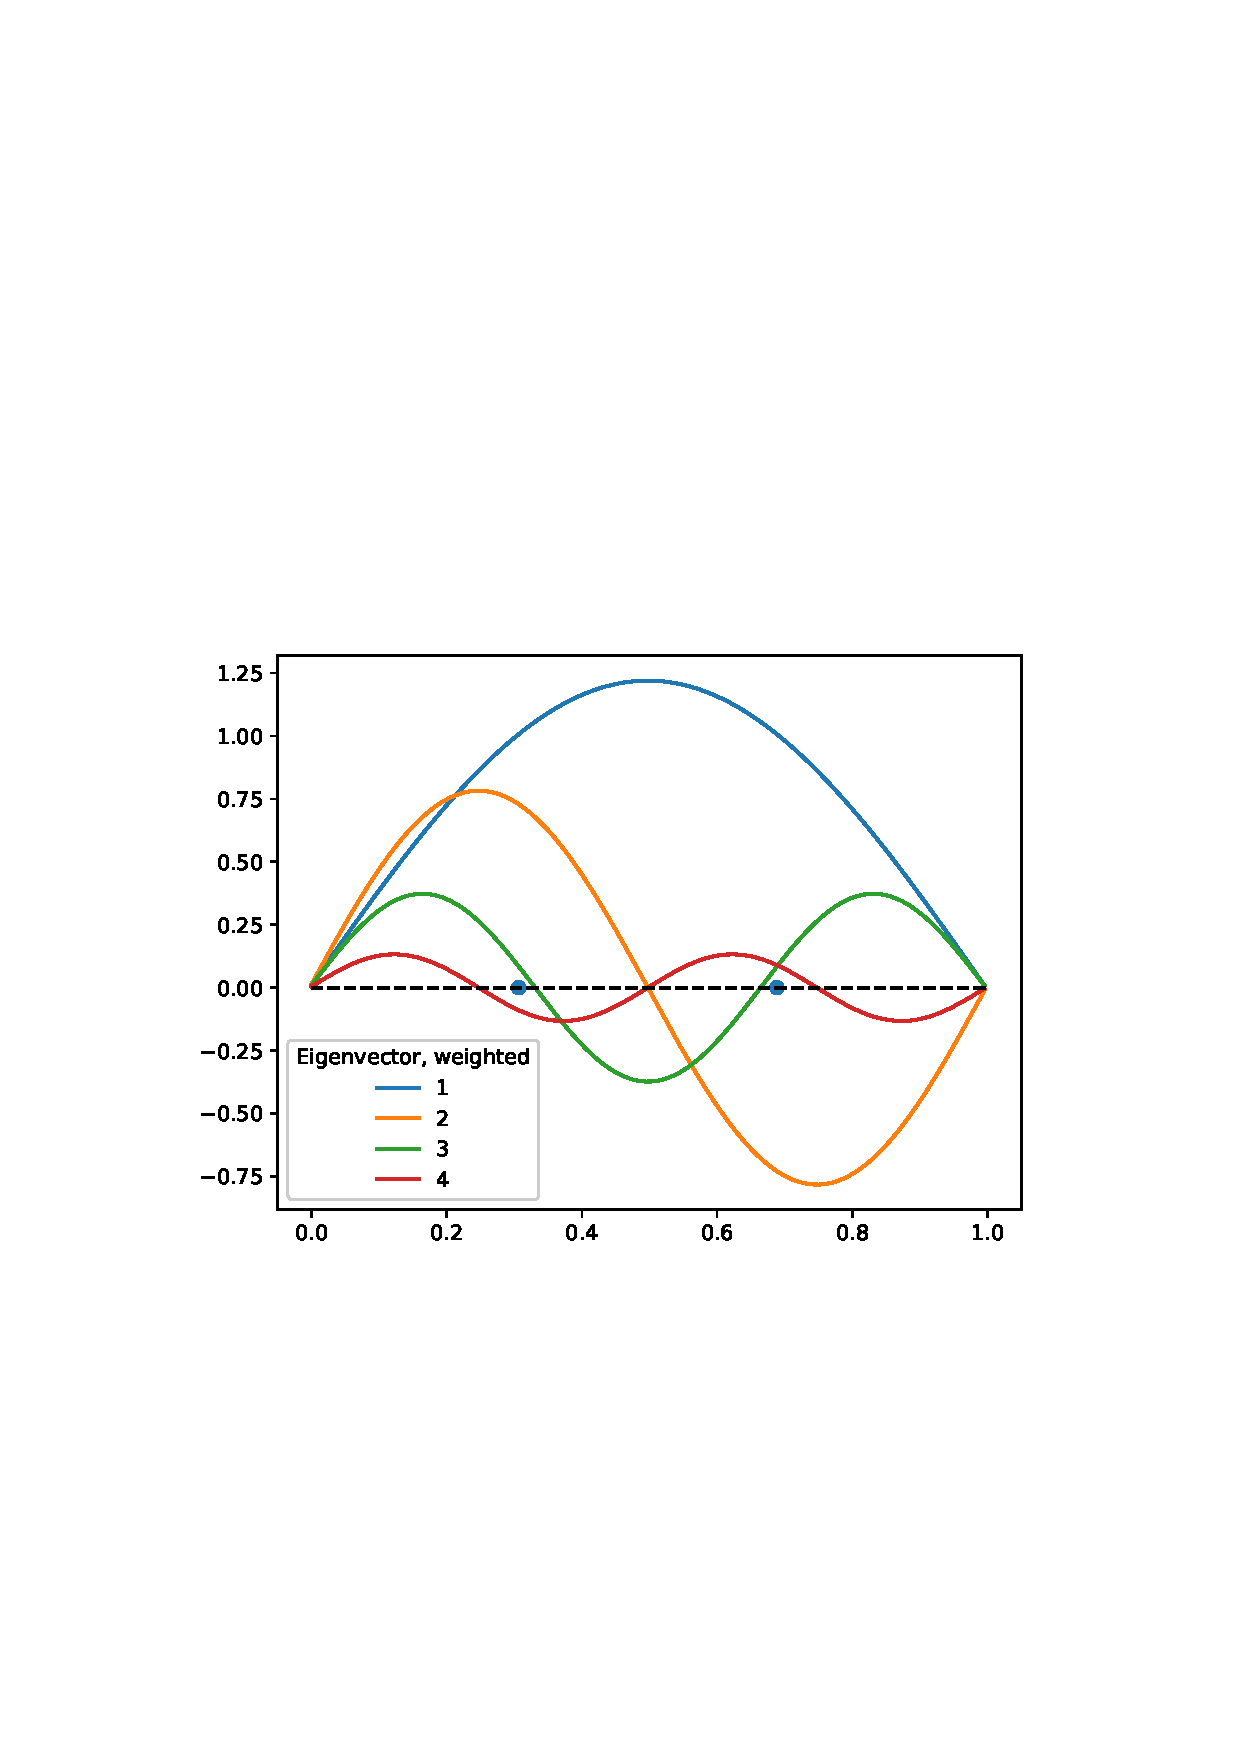
\includegraphics[height=0.5\textwidth]{eigenvectors.pdf}
    \caption{D-optimal measurement locations ($m=5$ measurements) and
      weighted eigenvectors for inversion of the initial condition of
      the 1D heat equation. Measurement locations and weighted
      eigenvectors are plotted over the computational domain $\Omega =
      [0, 1]$ (x-axis). Measurement clusterization occurs
      approximately at $0.31$ and $0.69$. These two locations are a
      compromise between zeros of eigenvectors a D-optimal design aims
      to ignore (third and up) and staying far from a zero of the
      first and second eigenvectors. Allocating $m=5$ measurements
      into two locations results in clusterization, according to the
      pigeonhole principle.}
  \label{fig:why}
\end{figure}


According to Theorem \ref{thm:char}, D-optimal designs aim to capture
a small subset of eigenvectors of the prior covariance, specifically
the $k$ eigenvectors with the highest prior variance. Our model
naturally achieves this objective by not measuring eigenvectors $k+1$
and above, as proven in Theorem \ref{thm:char}. Translating this
understanding to spatial problems, we anticipate that a D-optimal
design would favor measurement locations where eigenvectors $k+1$ and
above are either close to zero in value or possess small eigenvalues
in the prior spectrum, for some $k > 0$. To illustrate this
preference, Figure \ref{fig:why} depicts the scenario using the 1D
heat equation with homogeneous Dirichlet boundary conditions (details
in the supplementary material). The plot showcases four eigenvectors,
scaled according to their prior standard deviations. Since
eigenvectors beyond the fourth have insignificant prior eigenvalues,
we exclude them from consideration. Notably, we observe that
measurements are clustered near the zeros of the third and fourth
eigenvectors, so we conclude that $k=2$. Clusterization arises because
there are only two locations where the third and fourth eigenvectors
approach zero, while the first and second eigenvectors exhibit
significantly non-zero values. Consequently, when we allocate four
measurements to these two locations, they naturally cluster together,
aligning with the pigeonhole principle.


\section{Acknowledgements}
This study is a result of research I started during my PhD studies
under the instruction of Prof.~Georg Stadler at the Courant Institute
of Mathematical Sciences. I would like to thank him for his great
mentorship, attention to details and kindness. I would also like to
thank Christian Remling, who helped me find a proof for Lemma
\ref{lemma:free} in
\href{https://mathoverflow.net/questions/280168/redistribute-diagonal-entries-of-a-matrix/280203#280203c}{Mathoverflow}.
Last, but certainly not least, I would like to thank the three
referees, associate editor and editor in chief for providing detailed
and insightful reviewes that have made this manuscript a whole lot
better.
%Having worked on this manuscript alone for several years, they have
%almost become my coautoh

This research was supported in part by an appointment with the
National Science Foundation (NSF) Mathematical Sciences Graduate
Internship (MSGI) Program sponsored by the NSF Division of
Mathematical Sciences. This program is administered by the Oak Ridge
Institute for Science and Education (ORISE) through an interagency
agreement between the U.S. Department of Energy (DOE) and NSF. ORISE
is managed for DOE by ORAU. All opinions expressed in this paper are
the author's and do not necessarily reflect the policies and views of
NSF, ORAU/ORISE, or DOE.
% This work was also supported by The Raymond and Beverly Sackler
% Post-Doctoral Scholarship.


\bibliographystyle{amsplain}
\bibliography{/home/yair/projects/bibtex.bib}

\end{document}

%% %\section{Clusterization poses no obstruction to D-optimality}\label{section:clusterization}
\section{Substituting an optimal clustered design with an equally optimal non-clustered design}\label{section:how}
%
The necessary conditions for D-optimality of Theorem \ref{thm:char}
leave some freedom in choosing $\obs$, which might allow us to avoid a
clustered design. As an example, consider an inverse problem for which
the first two eigenvalues of the pushforward prior $\fwd \prcov\fwd^*$
are $\lambda_1 = 10, \lambda_2 = 5$, with eigenvectors
$\{\ev_i\}_{i=1}^\infty$ and $\sigma^2=1$. Consider the following
$\obs, \pobs$ (see also Fig.~\ref{fig:clusterization}):
\begin{equation}\label{eq:two designs}
  \obs =
  \begin{pmatrix}
    \sqrt{\frac{11}{40}}\ev_1 - \sqrt{\frac{29}{40}}\ev_2 \\
    \sqrt{\frac{11}{40}}\ev_1 + \sqrt{\frac{29}{40}}\ev_2 \\
    \ev_1 \\
    \ev_2 \\
    \ev_1 \\    
  \end{pmatrix},
  \pobs =
  \begin{pmatrix}
    \sqrt{\frac{3}{8}}\ev_1 - \sqrt{\frac{5}{8}}\ev_2 \\
    \sqrt{\frac{3}{8}}\ev_1 + \sqrt{\frac{5}{8}}\ev_2 \\
    \sqrt{\frac{2}{5}}\ev_1 - \sqrt{\frac{3}{5}}\ev_2 \\
    \sqrt{\frac{2}{5}}\ev_1 + \sqrt{\frac{3}{5}}\ev_2 \\
    \ev_1 \\    
  \end{pmatrix}
\end{equation}
\noindent It is easy to verify that $\obs^*\obs = \pobs^*\pobs$
and that both $\obs$ and $\pobs$ are D-optimal. However, $\obs$
is a clustered design ($\meas_3 = \meas_5 = \ev_1$), while $\pobs$ is
not.

We may now answer \textbf{Question \ref{q:replace}}: We showed that it
is possible to substitute a D-optimal clustered design (e.g. $\obs$)
for a D-optimal non-clustered design (e.g. $\pobs$). Presenting a
general algorithm for replacing a clustered D-optimal design with a
non-clustered D-optimal design is out of the scope of the current
study. We can, however, provide some intuition, utilizing $\obs,
\pobs$ as a test case. Let $\obs_{12}$ the design composed of the
first and second rows of $\obs$ (with a similar definition for
$\pobs_{12}$), and note that, up to permutations and sign changes,
$\obs_{12}$ uniquely determines $\obs$ as a clustered design. We find
$\pobs_{12}$ by requiring that (a) measurements in $\pobs_{12}$ have
unit norm, (b) $\pobs_{12}^* \pobs_{12}$ has the same eigenvectors as
$\obs^*\obs$, (c) $\pobs^*\pobs \approx \obs^*\obs$, and (d)
$\pobs^*\pobs \neq \obs^*\obs$. We then consider a ``new'' inverse
problem, for which the pushforward prior covariance is the covariance
of the posterior $\mu_{\textup{post}}^{\data, \pobs_{12}}$, namely

$$
\left(\left(\fwd \prcov\fwd^*\right)^{-1} + \sigma^{-2}
\pobs_{12}^*\pobs_{12}\right)^{-1}.
$$
%
Finally, we complete $\pobs$ to a D-optimal design with $m=5$
measurements via the construction outlined in Lemma
\ref{lemma:free}.

Interestingly, part (c) in the process detailed above implies that
there are actually infinitely many non-clustered D-optimal designs. It
is not at all clear why the numerical implementation of Lemma
\ref{lemma:free} results in a clustered design. An answer to this
question may further help shed light on the measurement clusterization
phenomenon.


\pgfplotstableread{
  Label    prior  $o_1o_2$  $o_3$   $o_4$   $o_5$    topper
  1         0.1      0.55       1       0       1      0.001
  2         0.2      1.45       0       1       0      0.001
  3         3.5      0          0       0       0      0.001
}\clusterization


\pgfplotstableread{
  Label    prior  $o_1o_2$  $o_3o_4$   $o_5$     topper
  1         0.1    0.75     0.8        1         0.001
  2         0.2    1.25     1.2        0         0.001
  3         3.5    0        0          0         0.001
}\noclusterization

\begin{figure}
  \begin{tikzpicture}[scale=0.85]
    \begin{axis}[
        ybar stacked,
        ymin=0,
        ymax=4,
        xtick=data,
        legend style={cells={anchor=east}, legend pos=north west, legend columns=-1},
        reverse legend=false, % set to false to get correct display, but I'd like to have this true
        xticklabels from table={\clusterization}{Label},
        xticklabel style={text width=2cm,align=center},
        legend plot pos=right,
        ylabel=precision --- prior and posterior,
        xlabel=eigenvector $i$,
      ]
    
      
      \addplot [fill=green!80]  table [y=prior, meta=Label, x expr=\coordindex] {\clusterization};
      \addplot [fill=blue!60]   table [y=$o_1o_2$, meta=Label, x expr=\coordindex] {\clusterization};
      \addplot [fill=red!60]    table [y=$o_3$, meta=Label, x expr=\coordindex] {\clusterization};
      \addplot [fill=black!60]  table [y=$o_4$, meta=Label, x expr=\coordindex] {\clusterization};
      \addplot [fill=orange!60] table [y=$o_5$, meta=Label, x expr=\coordindex] {\clusterization};
      %% \addplot [fill=cyan!60]   table [y=$o_6$, meta=Label, x expr=\coordindex] {\clusterization};
      %% \addplot [fill=purple!60] table [y=$o_7$, meta=Label, x expr=\coordindex] {\clusterization};

      
      \addlegendentry{prior}
      \addlegendentry{$o_1o_2$}
      \addlegendentry{$o_3$}
      \addlegendentry{$o_4$}
      \addlegendentry{$o_5$}
      %% \addlegendentry{$o_6$}
      %% \addlegendentry{$o_7$}   
    \end{axis}
  \end{tikzpicture}
  \qquad
  \begin{tikzpicture}[scale=0.85]
    \begin{axis}[
        ybar stacked,
        ymin=0,
        ymax=4,
        xtick=data,
        legend style={cells={anchor=east}, legend pos=north west, legend columns=-1},
        reverse legend=false, % set to false to get correct display, but I'd like to have this true
        xticklabels from table={\noclusterization}{Label},
        xticklabel style={text width=2cm,align=center},
        legend plot pos=right,
        ylabel=precision --- prior and posterior,
        xlabel=eigenvector $i$,
      ]
    
      
      \addplot [fill=green!80]  table [y=prior, meta=Label, x expr=\coordindex] {\noclusterization};
      \addplot [fill=blue!60]   table [y=$o_1o_2$, meta=Label, x expr=\coordindex] {\noclusterization};
      \addplot [fill=red!60]    table [y=$o_3o_4$, meta=Label, x expr=\coordindex] {\noclusterization};
      \addplot [fill=black!60]  table [y=$o_5$, meta=Label, x expr=\coordindex] {\noclusterization};
      %% \addplot [fill=orange!60] table [y=$o_4$, meta=Label, x expr=\coordindex] {\noclusterization};
      %% \addplot [fill=cyan!60]   table [y=$o_5$, meta=Label, x expr=\coordindex] {\noclusterization};
      %% \addplot [fill=purple!60] table [y=$o_6$, meta=Label, x expr=\coordindex] {\noclusterization};

      
      \addlegendentry{prior}
      \addlegendentry{$o_1o_2$}
      \addlegendentry{$o_3o_4$}
      \addlegendentry{$o_5$}
      %% \addlegendentry{$o_4$}
      %% \addlegendentry{$o_5$}
      %% \addlegendentry{$o_6$}   
    \end{axis}
  \end{tikzpicture}
  \caption{Clusterization (left, $\obs$ in \eqref{eq:two designs})
    and non-clusterization (right, $\pobs$ in \eqref{eq:two designs})
    in D-optimal designs. Posterior precision per eigenvector is
    plotted for $\obs$ and $\pobs$ from \eqref{eq:two
      designs}. Both designs are identical for all practical matters
    --- their posteriors are equal. In the left panel, a D-optimal
    design with clusterization is illustrated: $\meas_3 = \meas_5$. In
    the right panel, a D-optimal design without clusterization is
    illustrated. The contribution to the posterior precision due to
    $\meas_1$ and $\meas_2$ is denoted $\meas_1\meas_2$. These
    contributions are plotted together because neither $\meas_1$ nor
    $\meas_2$ are not in the direction of any eigenvector. Similarly
    for $\meas_3\meas_4$.}
  \label{fig:clusterization}
\end{figure}

%% \section{Open Problems}

